\pagebreak
\chapter{SQL}
\setcounter{section}{0}

\section{SQL - Conceptual}
On: Youtube
\subsection{Keys}

\subsubsection{Primäry Key}
Ein Primärer Schlüssel ist eine Spalte, welche jede Zeile in einer Tabelle eindeutig definiert. Dieser Schlüssel unterliegt dabei zwei Eigenschaften
\begin{itemize}
\item Eindeutigkeit (Unique)
\item Nicht Null (No Null)
\item Nicht änderbar (No changing)
\end{itemize}
Es wird dafür meist eine Identiätsspalte eingefügt, welche eine Indexierung vornimmt. Diese muss aber nicht zwangläufig der $"$Primäre Key$"$ sein.


\subsubsection{Composite Key}
Eine Tabelle, in welcher keine Spalte für sich eine eindeutige Identifikationsmöglichkeit darstellt, benötigt ein Composite Key. Dieser beinhaltet mindestens eine zwei Spaltenreferenzen. Diese Kombination aus Spalten ergibt eine Eindeutigkeit einer jeden Zeile. 

\begin{figure}[H]
	\centering
	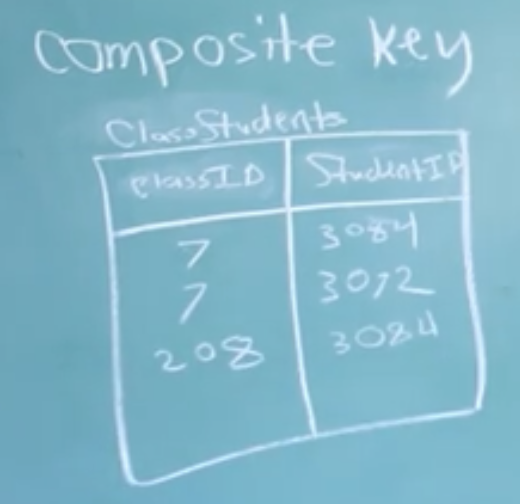
\includegraphics[scale = 0.3]{attachment/chapter_3/Scc030}
	\caption{}
	\label{fig:Scc030}
\end{figure}
In dem Beispiel ist erste jede Zeile identifizierbar, wenn ein Schlüssel aus beiden Spalten gebildet wird.


\subsubsection{Forgein Key}
Eine Tabelle, welche Werte aus einer anderen Tabelle abfragt, benötigte eine Referenz zu dieser benötigten Tabelle. Die Tabelle, aus der Werte benötigt werden, fällt unter der Kategorie \textbf{Eltern}. Die Tabelle, welche Werte aus der Eltern Tabelle benötigt, fällt unter der Kategorie \textbf{Kind}.\\

In dem Fall, dass eine Kind Tabelle eindeutige Zeile in der Eltern Tabelle referieren muss, wird ein \textbf{Forgein Key} benötigt. Dieser muss
\begin{itemize}
\item nicht null sein,
\item eindeutig die Eltern Tabelle referieren.
\end{itemize}
Es ist jedoch möglich eine einen null Eintrag in der Forgein Key Spalte zu besitzen, welche nicht zur Spalte der Eltern Tabelle referiert. Daraus folgt, dass der Forgein Key nicht eindeutig sein muss und null sein kann. Diese ist ein Adopiv-Kind, welches nicht zu einer zu einer gewissen Zeile in der Primärschlüssel Spalte der Elterntabelle referiert. 
\subsubsection{Composite Key}
Wenn eine Tabelle zugrunde liegt, in welcher keine Spalte für sich als Primär Key fungiert, so wird eine Primär Key oder auch Composite Key aus mehreren Spalten gebildet.

In der Tabelle mit Studenten-ID und Class-ID, gibt eis keinen Primären Schlüssel. Die Spalten müssen verbunden werden, sodas ein eindeutiger Schlüsel für die Tabelle geschaffen wird. 
\begin{figure}[H]
	\centering
	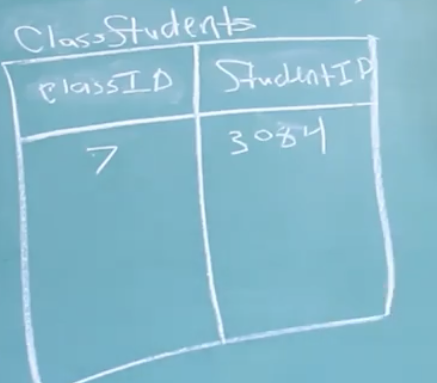
\includegraphics[scale = 0.3]{attachment/chapter_3/Scc031}
	\caption{}
	\label{fig:Scc031}
\end{figure}


Es kann nämlich sein, dass in der Spalte mehrere gleiche Werte stehen.

\begin{figure}[H]
	\centering
	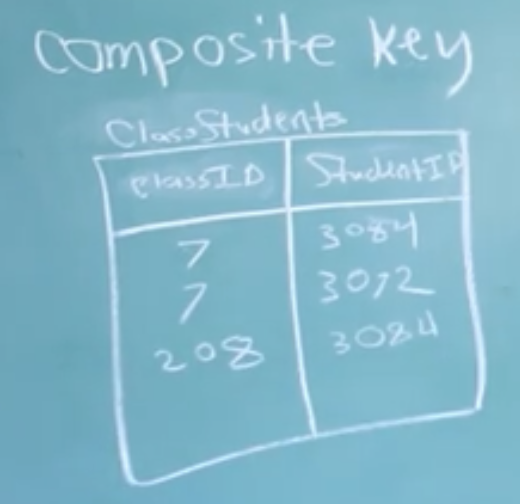
\includegraphics[scale = 0.3]{attachment/chapter_3/Scc030}
	\caption{}
	\label{fig:Scc030}
\end{figure}

Ein Composite Key ist somit ein Primäry Key, welcher sich über mehrer Spalten erstreckt.

\subsubsection{Compound Key}
Ein Compound Key ist fast gleich zum Composite Key mit dem Unterschied, dass die verbundenen Spalten selber wieder Forgein Key sind, und somit zu anderen Tabellen verweisen.

\begin{figure}[H]
	\centering
	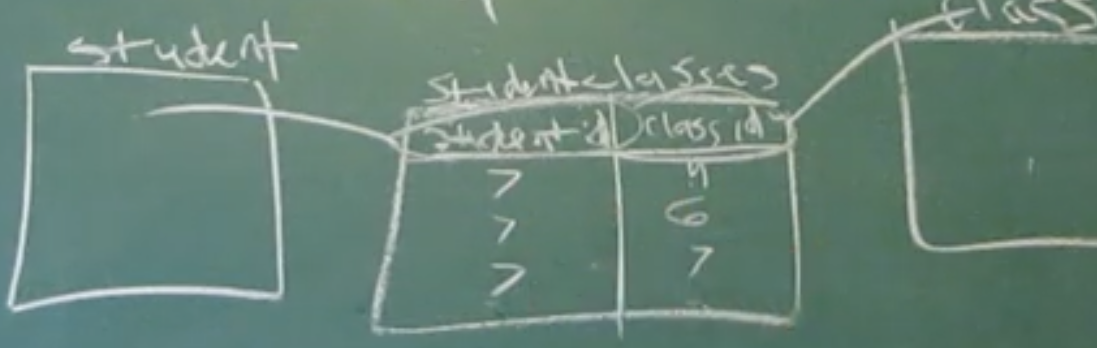
\includegraphics[scale = 0.3]{attachment/chapter_3/Scc032}
	\caption{}
	\label{fig:Scc032}
\end{figure}

\subsection{Normilization}
\subsubsection{1NF - Atomicity}
In diesem Kontext wir von Entities und Attributes gesprochen. Dabei werden Entities in Tabellen umgesetzt und Attributes als Spalten definiert. 
Die Atomizierung beschriebt, dass die Zielsetzung einer Tabelle sind in der Wahl der Spalten niederschlagen soll. Das bedeutet, Werte in der Spalte mit dem Hauptbezug keine mehreren Werte besitzen soll. In anderen Spalten sind wiederkehrende Werte akzeptable. In anderen Hauptbezug-Spalte/ Spalten ist dies nicht akzeptable. Der Primärkey ist damit jedoch nicht zwangsläufig gemeint.\\

Wenn einem Instanz einer Tabelle mehrer Werte zugeordnet werden müssen, dann sollte dies in einer ergänzenden Tabelle geschehen, welche den Hauptzweck besitzt, das Attribute abzugedecken. Jedoch gilt auch hier, dass Eindeutigkeit benötig wird. 

\begin{figure}[H]
	\centering
	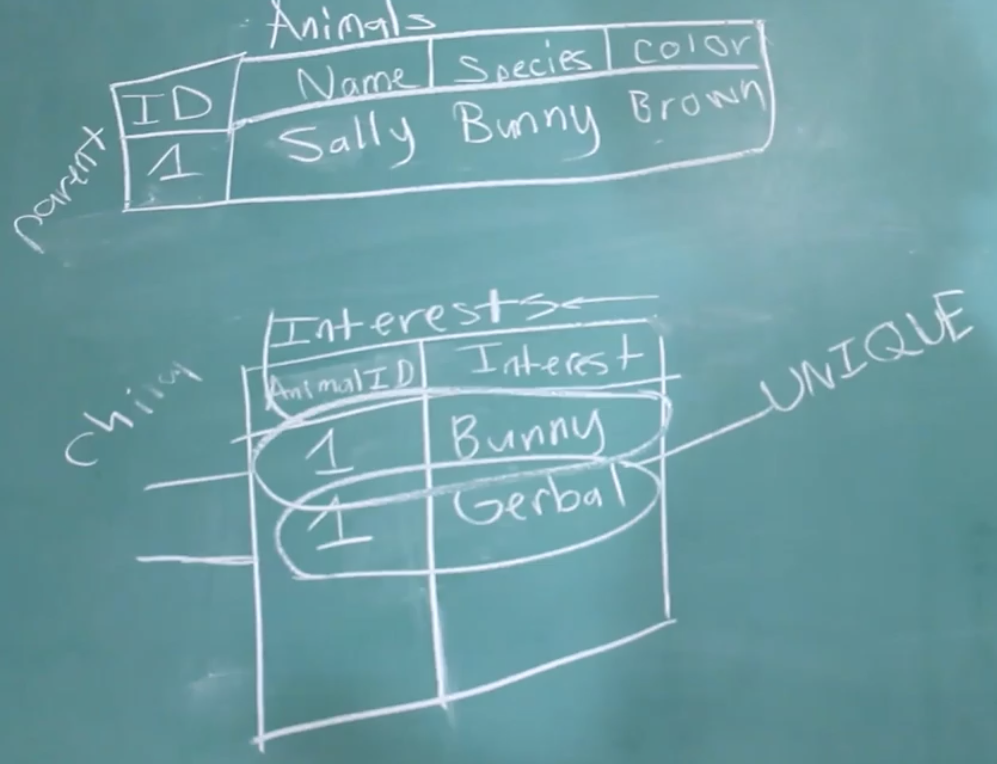
\includegraphics[scale = 0.3]{attachment/chapter_3/Scc034}
	\caption{}
	\label{fig:Scc034}
\end{figure}
Am Beispiel zeigt sich, dass Interests verwendet wird, Interessen für verschiedene Tiere zu speichern. Dabei kann ein Tier mehrere Interessen haben, jedoch in jeder Zeile steht nur ein Tier mit einem eindeutigen Interesse.
\begin{center}
Eine Tabelle befindet sich in 1Nf, 
\begin{itemize}
\item wenn ein oder mehrer Attribute kein Duplikat eines anderen Attributes ist.
\item wenn Instanzen eines Attributes keine Gruppierung des zugehörigen Attributes ist.
\end{itemize}
\end{center}

Das bedeutet, dass mehrere Ausprägungen eines Attributes nicht in einer Tabelle stehen sollen. Ebenso sollten auch diese auch nicht in einer Zelle gruppiert stehen. Diese sollen eindeutige Einträge in eine weitere Tabelle übertragen werden.

\begin{figure}[H]
	\centering
	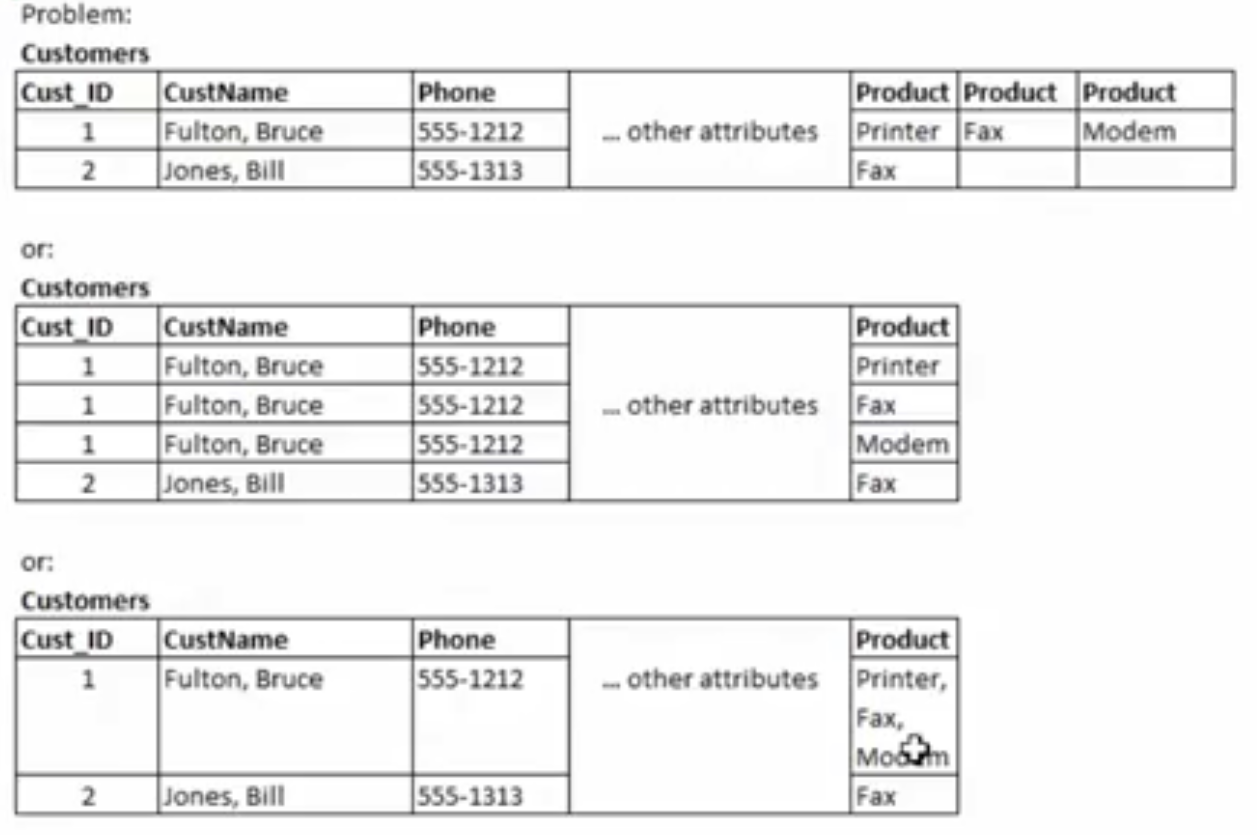
\includegraphics[scale = 0.3]{attachment/chapter_3/Scc033}
	\caption{}
	\label{fig:Scc033}
\end{figure}

Die Lösung zu dem Problem kann sein, dass eine Junction Tabelle erstellt wird.

\begin{figure}[H]
	\centering
	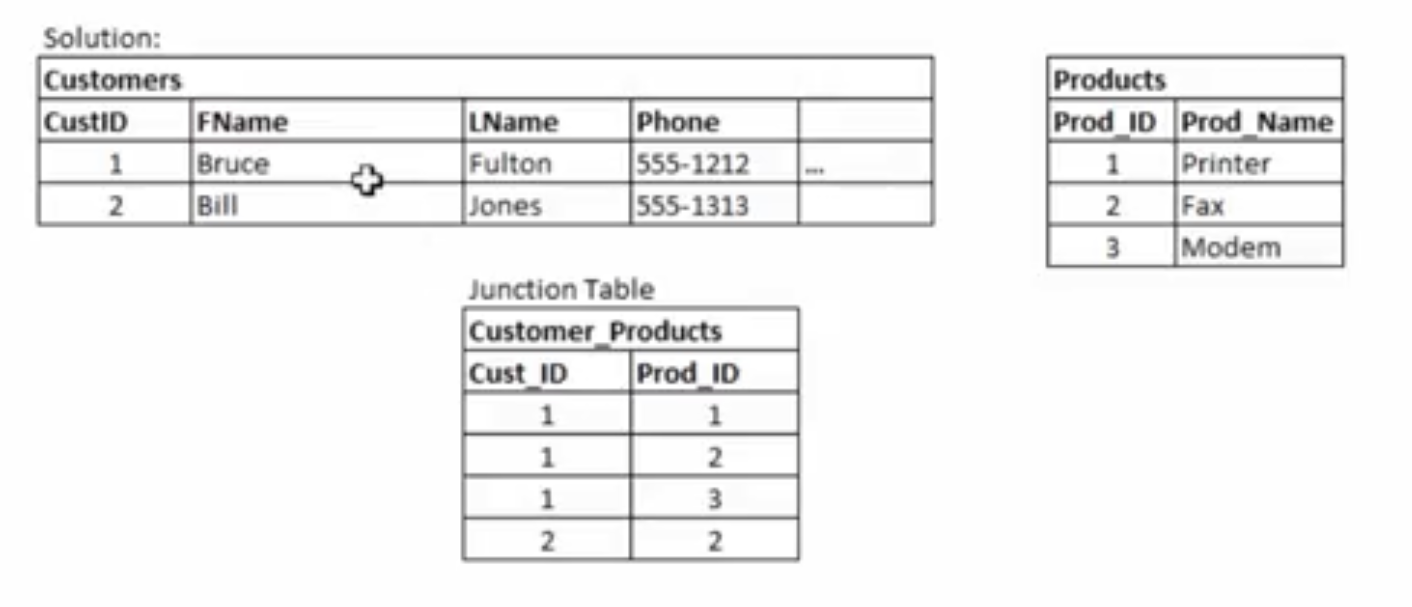
\includegraphics[scale = 0.3]{attachment/chapter_3/Scc035}
	\caption{}
	\label{fig:Scc035}
\end{figure}
Eine Juncion Tabelle wird nicht benötigt, wenn die ausgegliederte Tabelle sich nicht vollständig auflisten lässt.

\subsubsection{2NF - Partial Dependency}
Die zweite Normalisierung setz die erste voraus. Als weiteren Punkt müssen alle Non-Key Attributes sich auf den Primäre Schlüssel beziehen. Bei einem Primären Key, welcher aus einer Spalte besteht, ist 2NF gleich 1NF. 

In einer Tabelle, welche einen Compoud Key besitzen, müssen sich alle Non-Attribute auf alle Bestandteile des Primären Key beziehen. Im folgenden Beispiel ist dies nicht gegeben.

\begin{figure}[H]
	\centering
	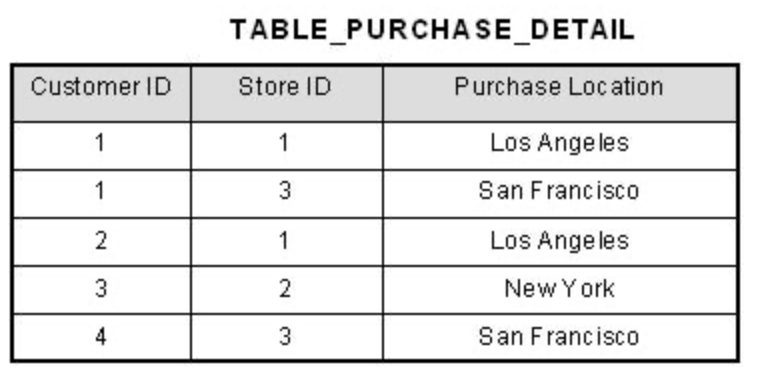
\includegraphics[scale = 0.3]{attachment/chapter_3/Scc036}
	\caption{}
	\label{fig:Scc036}
\end{figure}
Mit Hilfe der 2NF wir entweder die Tabelle getrennt oder die Daten nicht extra mit einbezogen.

\begin{figure}[H]
	\centering
	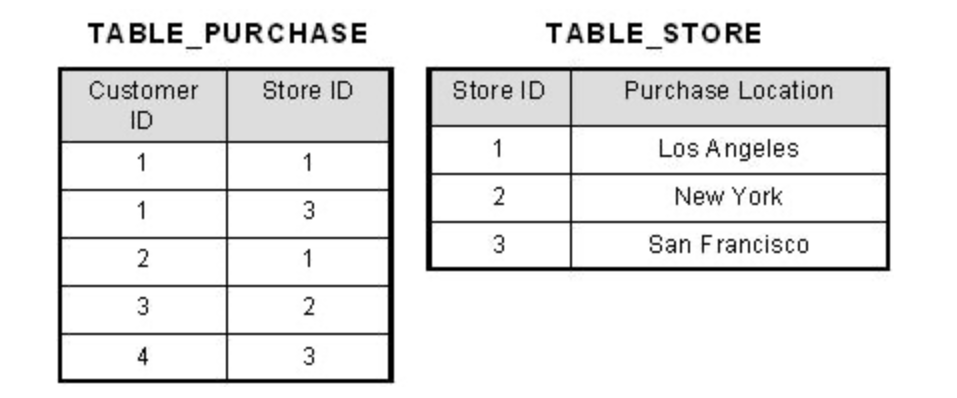
\includegraphics[scale = 0.3]{attachment/chapter_3/Scc037}
	\caption{}
	\label{fig:Scc037}
\end{figure}

\subsubsection{3NF - Transitive Dependency}
Die dritte Normalisierung setzt sich aus den beiden vorherigen zusammen. Aufbauend auf das vorherige folgt, dass ein Non-Key Attribute sich nicht auf ein anderes Non-Key Attribute beziehen soll.

\begin{figure}[H]
	\centering
	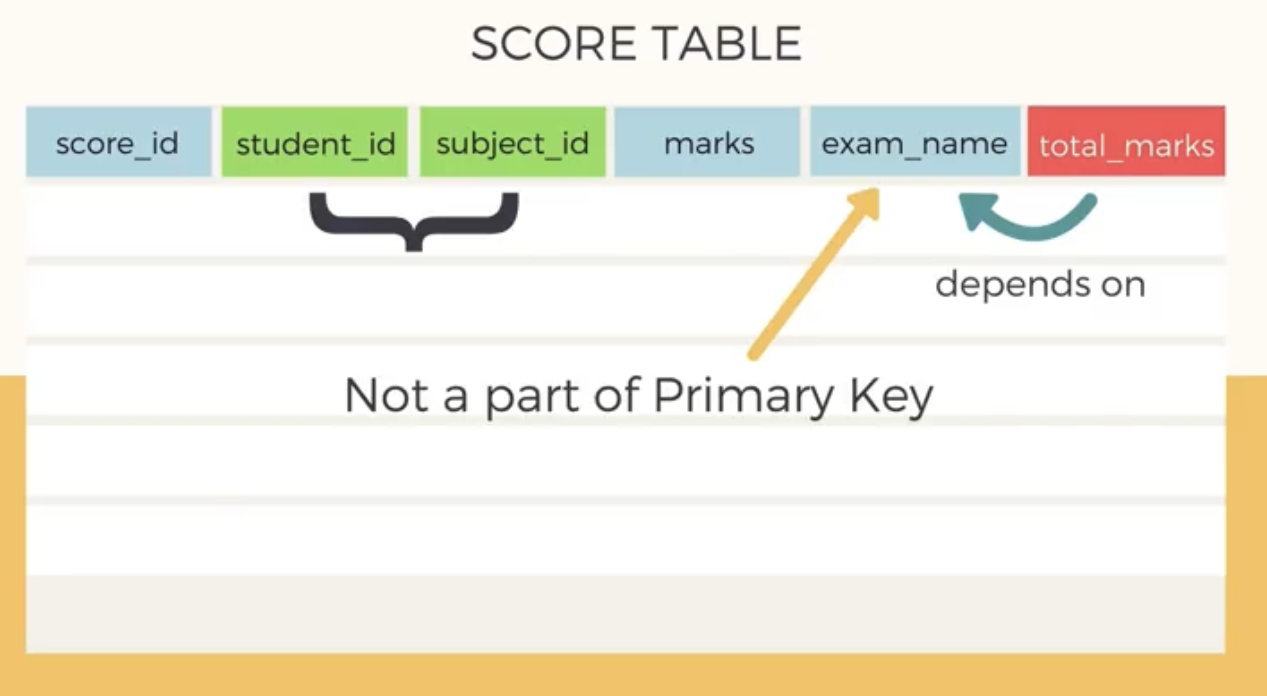
\includegraphics[scale = 0.3]{attachment/chapter_3/Scc038}
	\caption{}
	\label{fig:Scc038}
\end{figure}
Die gesamt Anzahl der Punkte ist Abhängig von der Art des Test. Diese Information sollte ausgeliedert werden.


\begin{figure}[H]
	\centering
	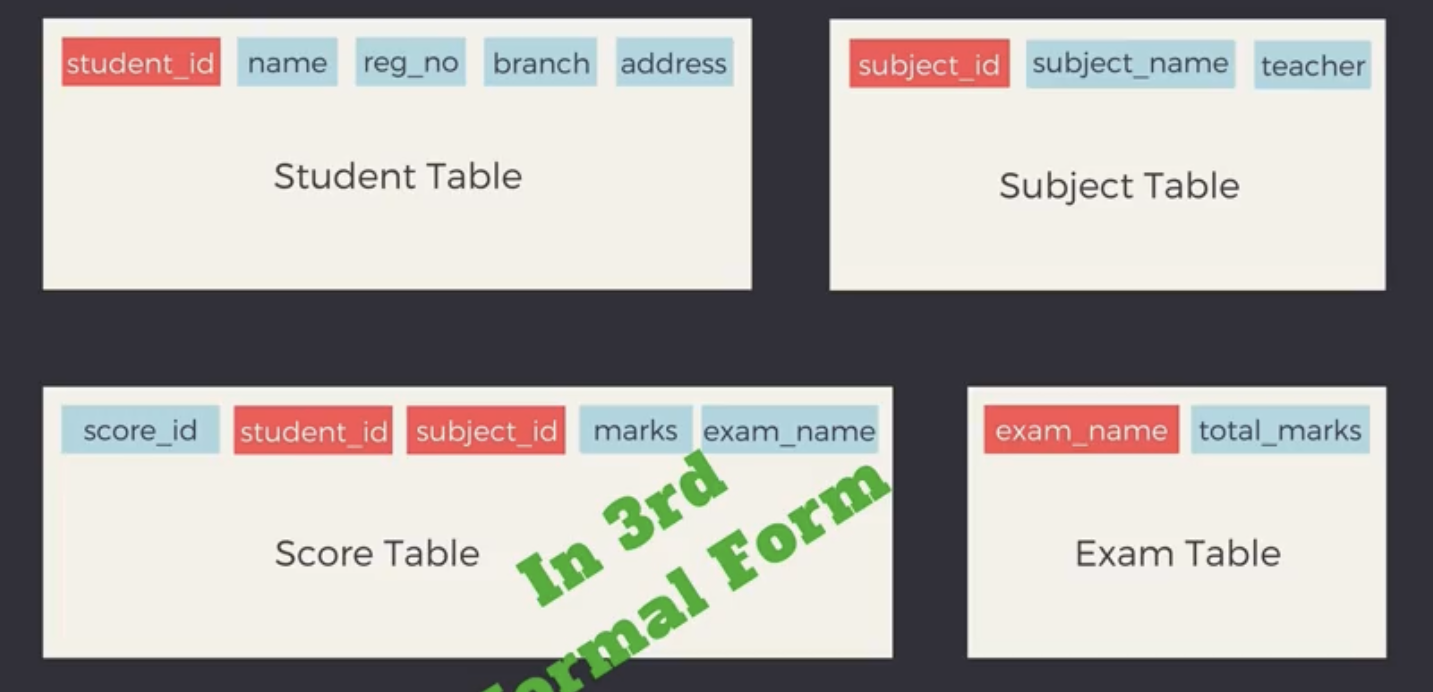
\includegraphics[scale = 0.3]{attachment/chapter_3/Scc039}
	\caption{}
	\label{fig:Scc039}
\end{figure}

\subsection{Junction}
\subsubsection{One-to-One Relationship}
Trival.
\subsubsection{One-to-Many Relationship}
Trival.
\subsubsection{Many-to-Many Relationship}
Um eine Beziehung zwischen zwei Primärkeys herzustellen, welche in einer Many-to-Many Beziehung stehen, benötigt es eine intermediären Tabelle.
In dieser besteht in keiner der Foreign Key Spalten eine Eindeutigkeit.

Am Beispiel der Beziehung zwischen Autorinnen und Büchern lässt sich zeigen, dass es eines zwei One-to-Many Beziehungen benötigt, um eine Many-to-Many Beziehung abzubauen.
\begin{figure}[H]
	\centering
	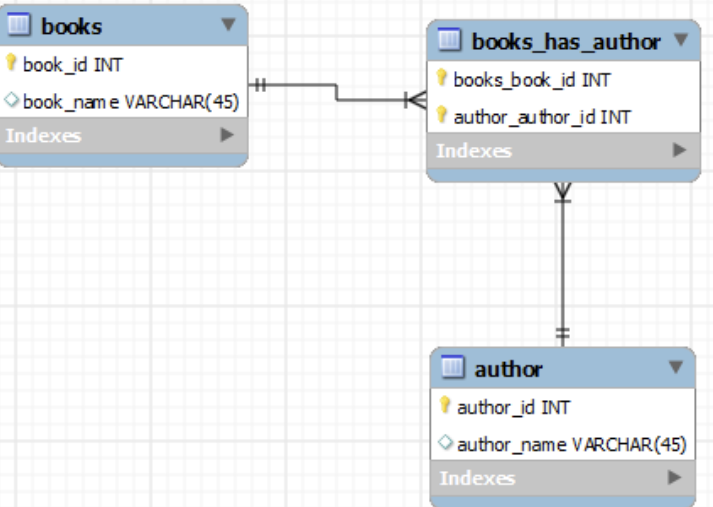
\includegraphics[scale = 0.3]{attachment/chapter_3/Scc040}
	\caption{}
	\label{fig:Scc040}
\end{figure}

Die Autorinnen können mehrere Bücher verfasst werden. Die Bücher können mehrer Autorinnen haben. In der Junction Tabelle wird die Permutation dargestellt, ohne dabei eine Tabelle zu erzeugen, in welcher mehrere Attribute von einem abgeleitet werden.

\subsection{Data Integrity}
Daten Integrität befasst sich mit Frage, wie können Datenbanken eine gewisse Stabilität und Verlässlichkeit gewähren. Dabei werden die vorherigen beschriebenen Themen verwendet.
Daten Integrität lässt sich in drei Bereiche aufteilen.
\begin{itemize}
\item Entry Integrity
\item Reference Integrity
\item Domain Integrity
\end{itemize}

Die erste beiden nutzen als Grundlage die Primär und Foreign Keys.

\begin{figure}[H]
	\centering
	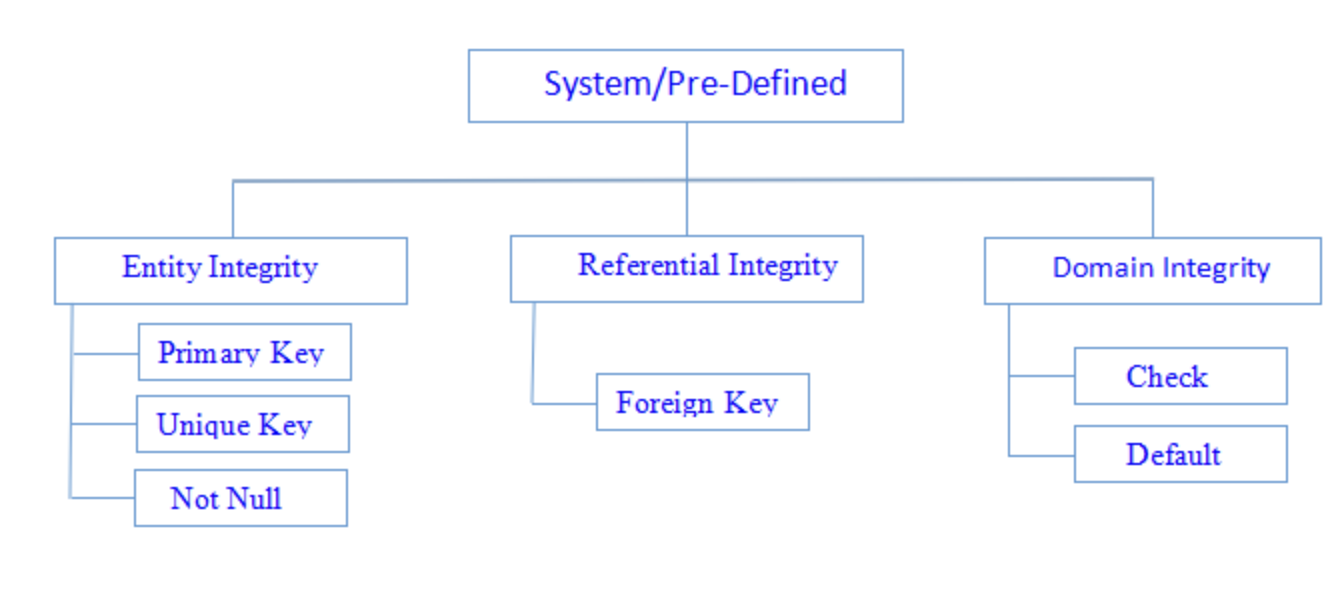
\includegraphics[scale = 0.3]{attachment/chapter_3/Scc041}
	\caption{}
	\label{fig:Scc041}
\end{figure}

Domain Integrity beschäftig sich damit, das Einträge in die Tabellen die richtigen Formate und Rahmenbedinungen (Constrains) erfüllen. 


\section{SQL - Introduction}
On: LinkedInLearning
Eine Relational Database ist eine DB, in welcher Informationen in zweidimensionale Tabellen gespeichert werden.


\subsection{SELECT Statment}
Soll eine komplette Tabelle bezogen werden, so wird das Sternchen * verwendet. In der Beispieldatenbank befindet sich die Tabelle Countrys.
Sollen alle Spalten und Wert der Tabelle bezogen werden, wird * verwendet, um alle Spalten der Tabelle auszuwählen:

\begin{lstlisting}[style=SQL]
SELECT *
From Customers;
\end{lstlisting}

\begin{figure}[H]
	\centering
	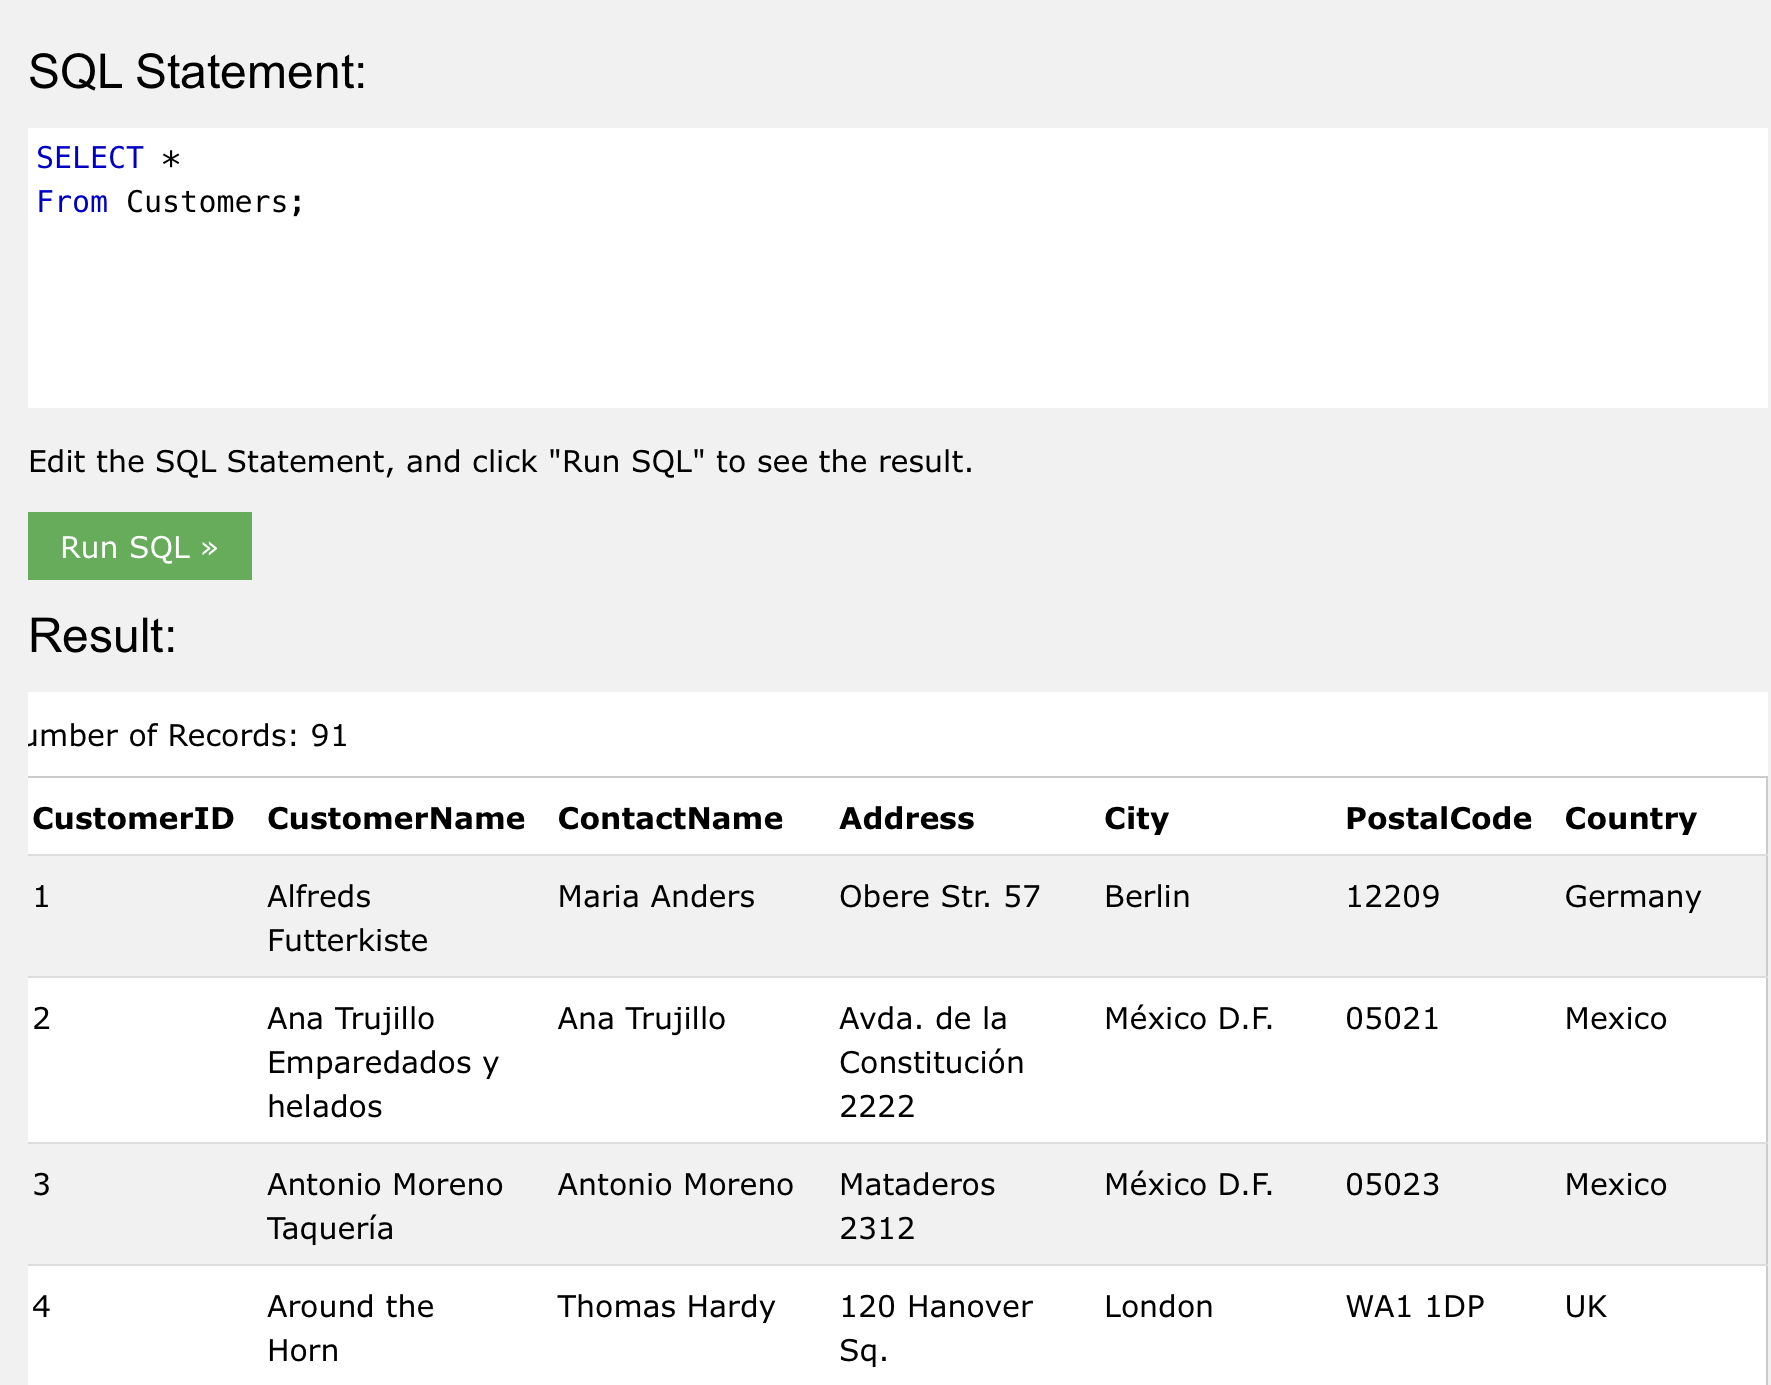
\includegraphics[scale = 0.3]{attachment/chapter_3/Scc048}
	\caption{}
	\label{fig:Scc048}
\end{figure}

Ein Teilmenge der Spalten wird über die genaue Adressierung angesteuert.
Die Interne Ordnung legt dabei die Reihenfolge der Spalten in der übergebenen Tabelle fest.

\begin{lstlisting}[style=SQL]
SELECT CustomerID, Adress
From	Customers;
\end{lstlisting}

\begin{figure}[H]
	\centering
	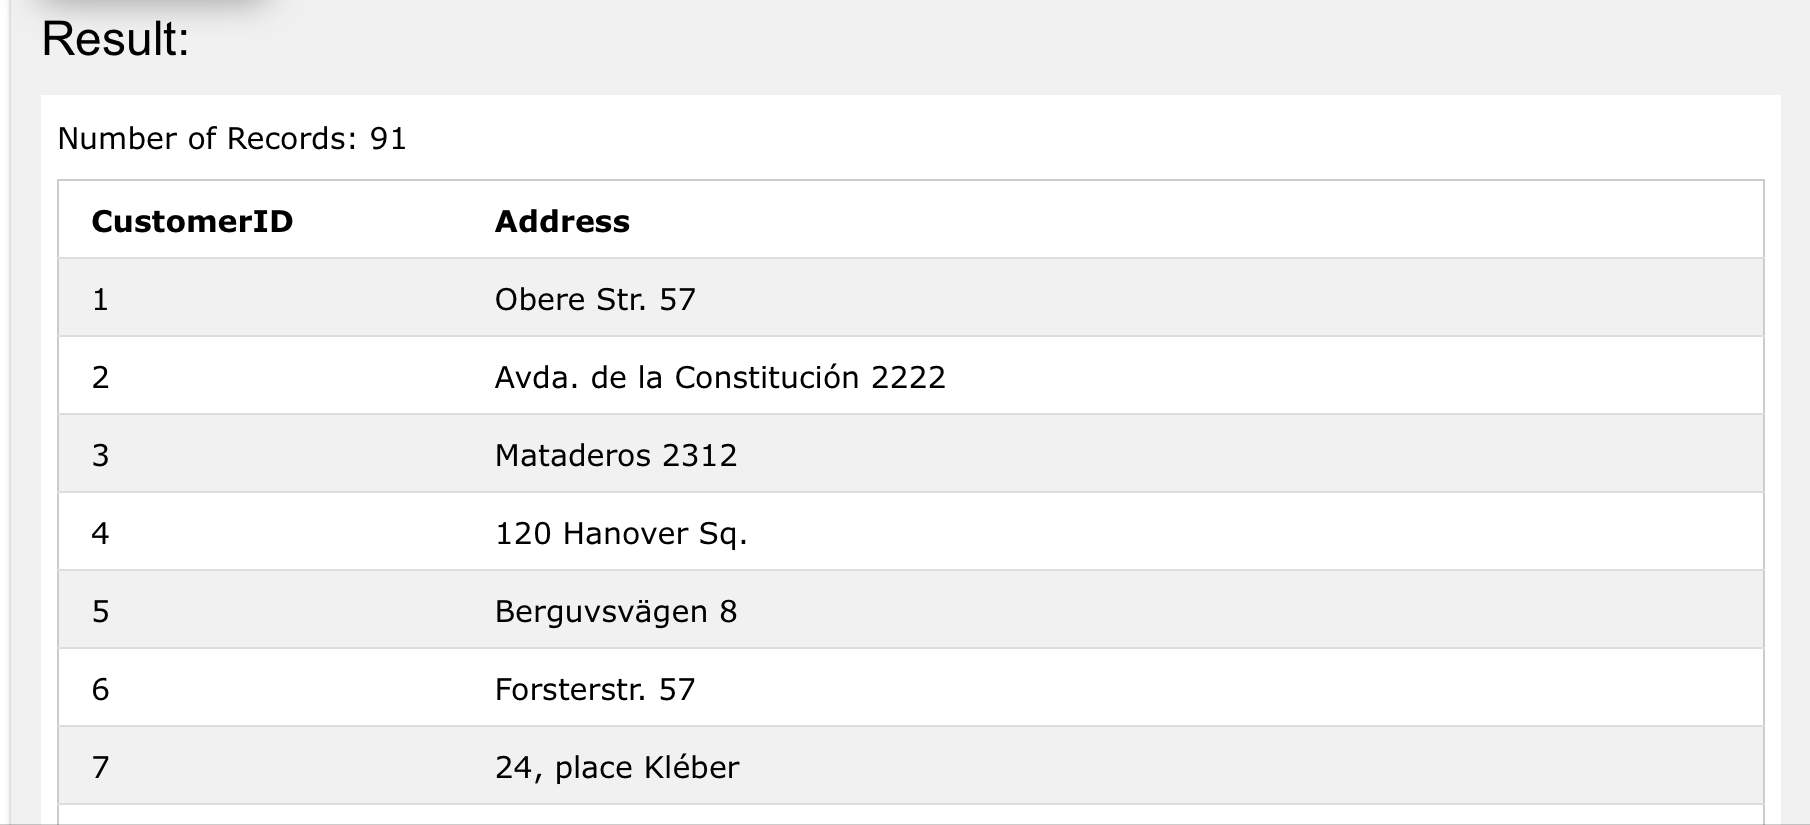
\includegraphics[scale = 0.3]{attachment/chapter_3/Scc049}
	\caption{}
	\label{fig:Scc049}
\end{figure}

Wie unten beschrieben, können die Bezeichnungen der Spalten durch \bl{AS} geändert werden.

\begin{lstlisting}[style=SQL]
SELECT CustomerID AS Index, Adress
From	Customers;
\end{lstlisting}

\begin{figure}[H]
	\centering
	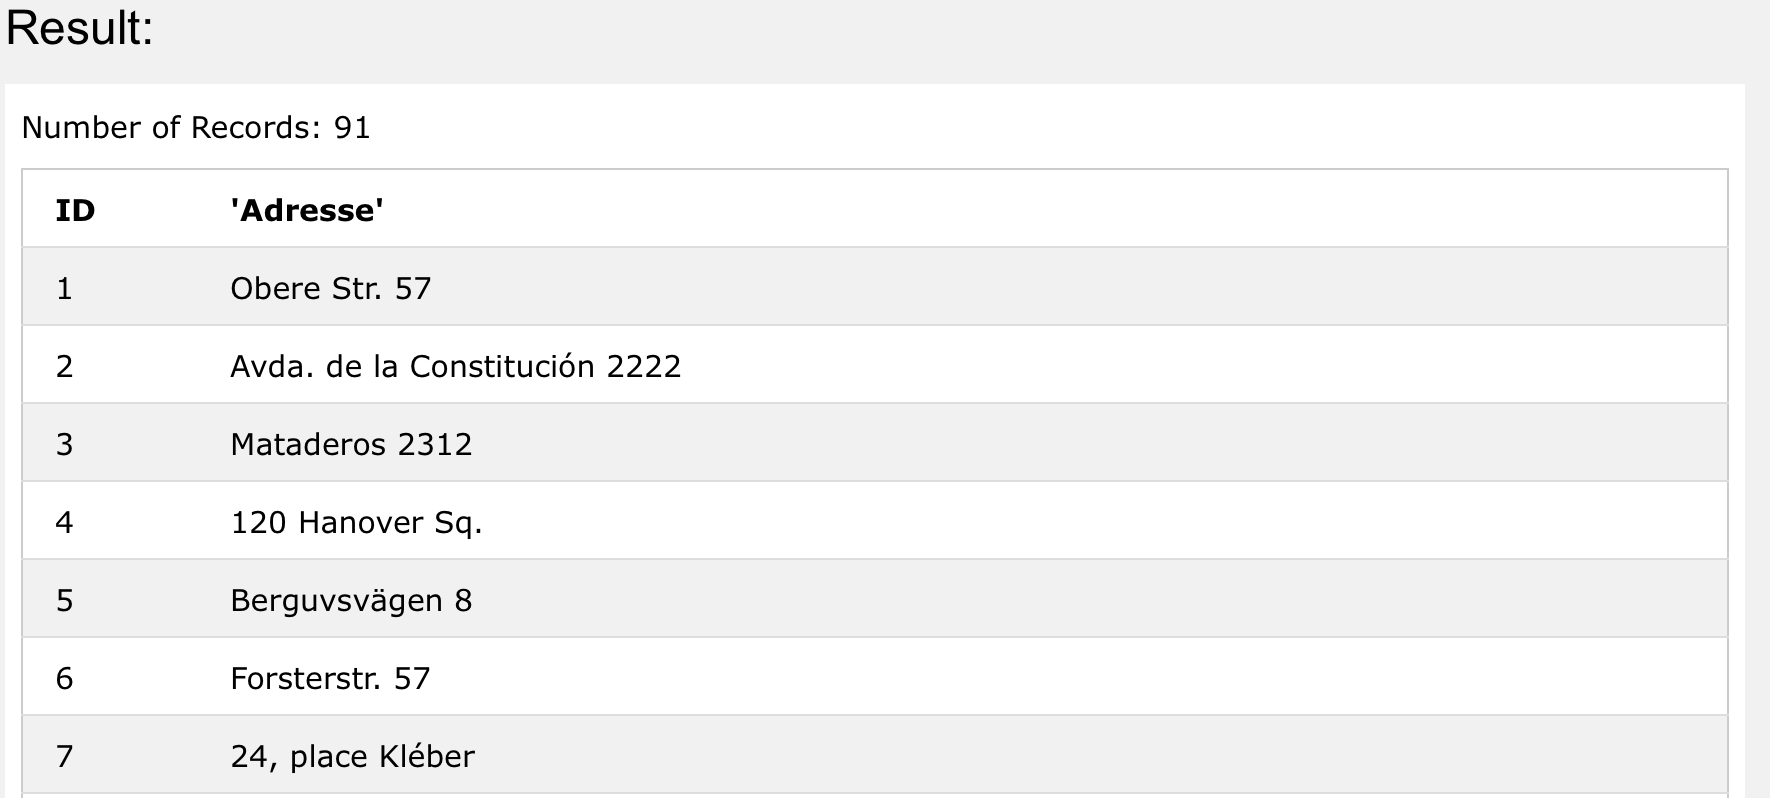
\includegraphics[scale = 0.3]{attachment/chapter_3/Scc050}
	\caption{}
	\label{fig:Scc050}
\end{figure}

Für die Dauer der Abfrage kann der Spaltennamen und oder der Tabellennamen, der genierten Tabelle, mit \bl{AS} geändert werden.

\begin{lstlisting}[style=SQL]
SELECT CustomerID AS ID, Address As 'Adresse'
From Customers;
\end{lstlisting} 

\begin{figure}[H]
	\centering
	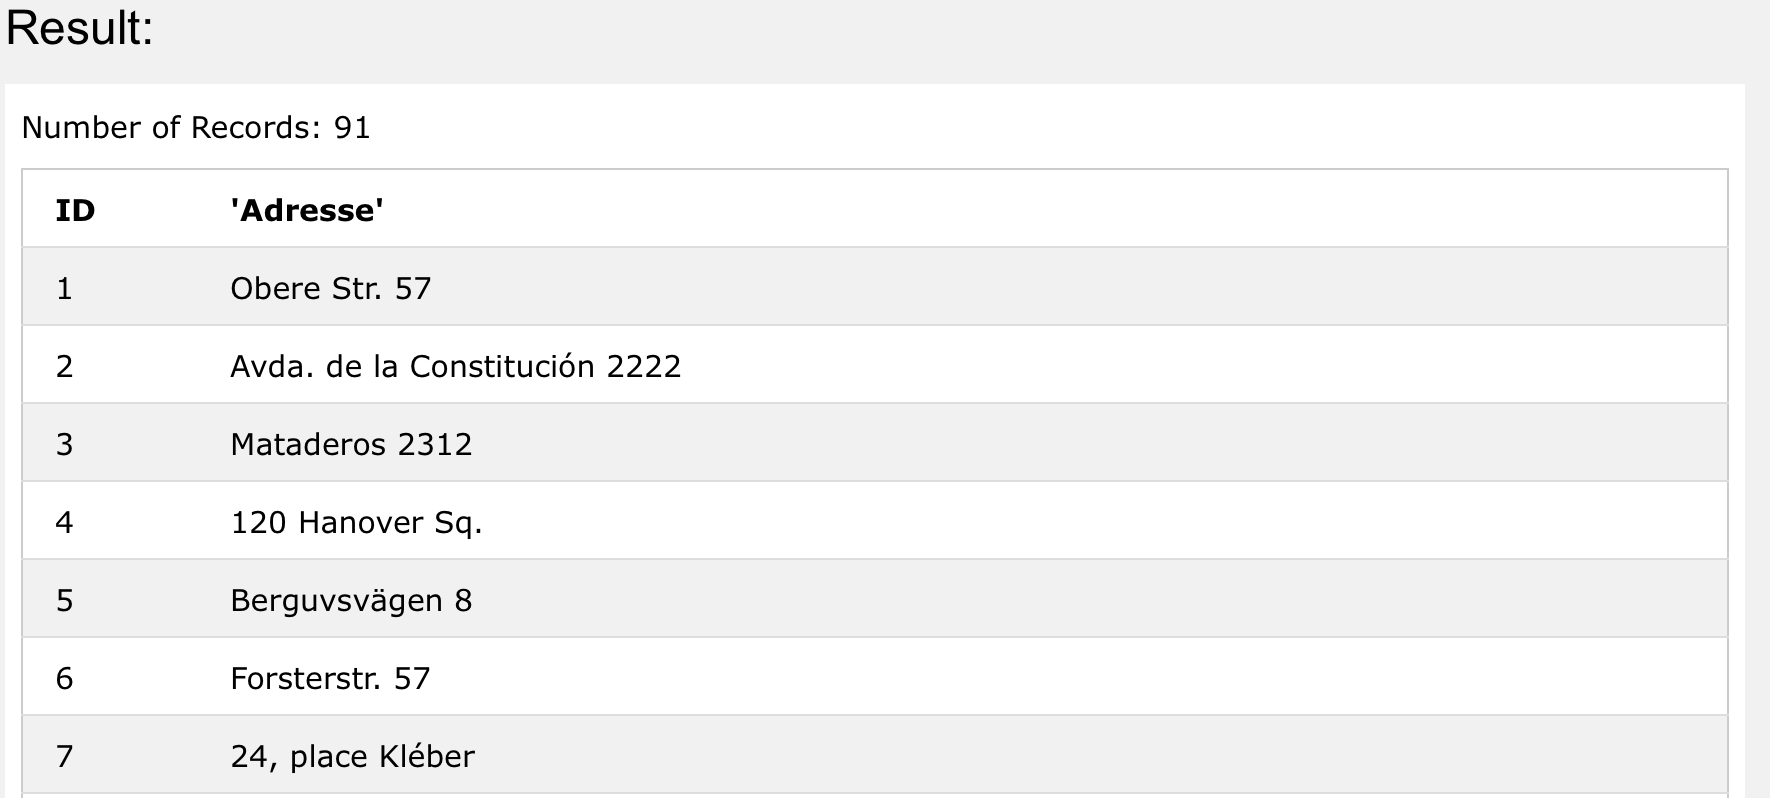
\includegraphics[scale = 0.3]{attachment/chapter_3/Scc050}
	\caption{}
	\label{fig:Scc050}
\end{figure}

Mit Apostrophen können auch Schlüsselwörter als Spaltennamen verwendet werden.

\subsubsection{FROM - Input table}
Mit \bl{FROM} wir die Quelle der SQL Anfrage bestimmt. Dies kann eine einfache Tabelle sein oder auch Tabelle, welche \bl{Joins} zu anderen Tabellen besitzt.

\subsubsection{WHERE - Where row is evaluated}
Die Clause \bl{WHERE} ist besser im Englischen zu verstehen. 
Select the following rows \bl{where} $\dots$ are equal to $\dots$.

\begin{lstlisting}[style=SQL]
SELECT *
FROM Customers
WHERE City = 'Berlin';
\end{lstlisting}

\begin{figure}[H]
	\centering
	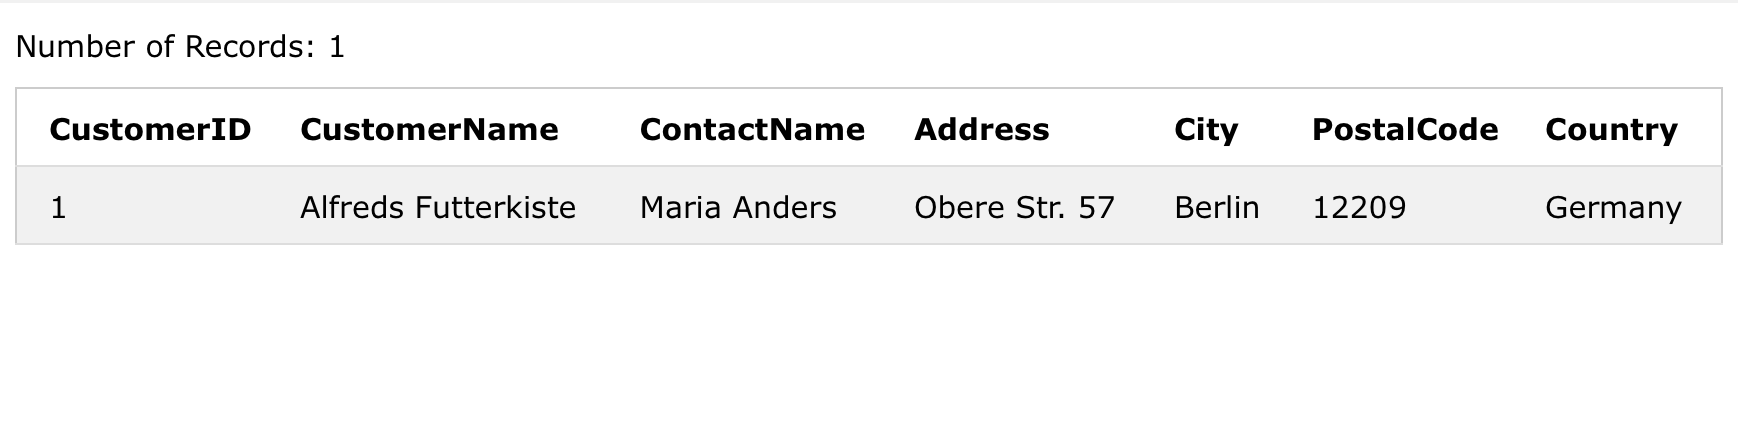
\includegraphics[scale = 0.3]{attachment/chapter_3/Scc044}
	\caption{}
	\label{fig:Scc044}
\end{figure}

Es kann auch nach einzelnen Begriffen gesucht werden. Mit \bl{Like} kann nach einzelnen Begriffen gesucht werden. 
\begin{itemize} 
\item Mit $\%$ können Begriffe einzeln betrachtet werden.
\item Mit $'\%\dots\%'$ wird der Begriff gesucht, egal was davor oder danach steht.
\item Mit $'\%\dots'$ wird der Begriff gesucht, egal was davor steht.
\item Mit $'\dots\%'$ wird der Begriff gesucht, egal was danach steht.
\end{itemize}

Ebenso können einzelnen Buchen an gewissen Stellen gesucht werden. Dafür nutzt man $\_$.

\begin{lstlisting}[style=SQL]
SELECT Country
FROM Customers
WHERE Name Like '%Tim%' // Anfang oder Ende ist egal.
\end{lstlisting}

\begin{lstlisting}[style=SQL]
SELECT Country
FROM Customers
WHERE Name Like '_i%' // Zweites Zeichen ist i
\end{lstlisting}

Um mehrer Bedingungen festzulegen, wird der \bl{IN()} Operator festgelegt. 

\begin{lstlisting}[style=SQL]
SELECT Country
FROM Customers
WHERE Name IN('West', 'Ost')
\end{lstlisting}


\subsubsection{GROUP BY - zusammenfassen von Spalten}
Im einfachen Fall wird diese Clause genutzt um eindeutige Werte einer Spalte auszugeben.

\begin{lstlisting}[style=SQL]
SELECT Country
FROM Customers
GROUP BY Country
\end{lstlisting}

\begin{figure}[H]
	\centering
	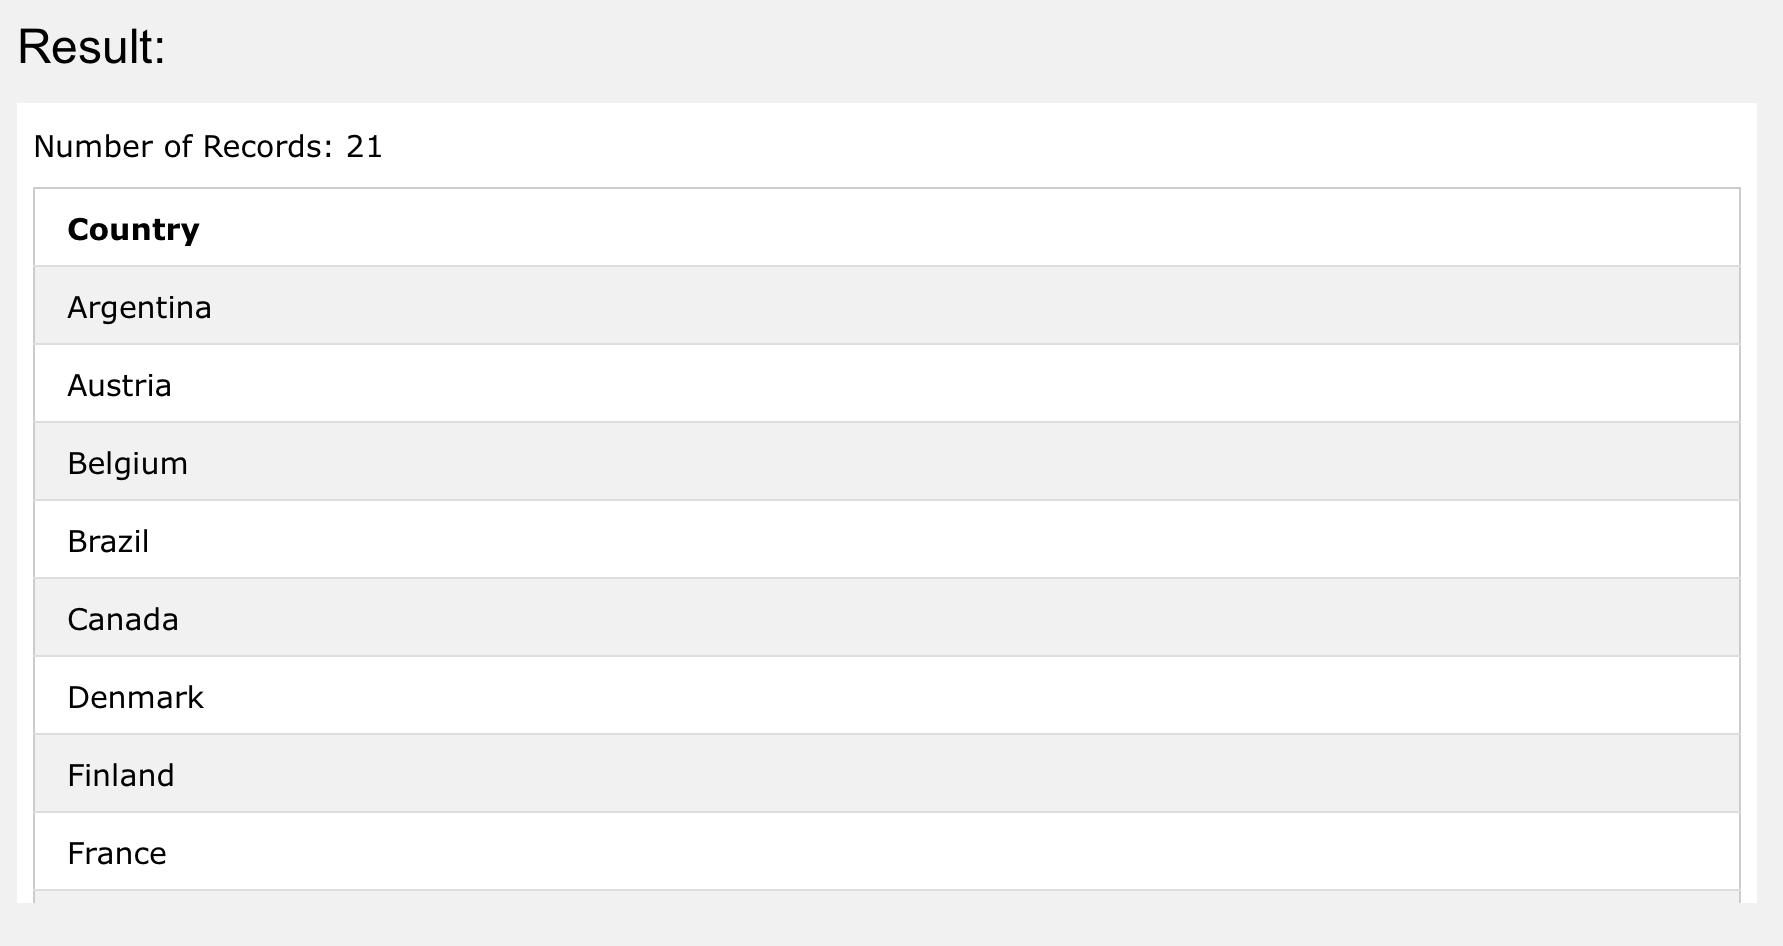
\includegraphics[scale = 0.3]{attachment/chapter_3/Scc047}
	\caption{}
	\label{fig:Scc047}
\end{figure}

\subsubsection{ORDER BY - sort table}
Zum Ordnen einer Tabelle wird \bl{Order by} verwendet. Danach wir der Spaltennamen eingetragen, nach dem absteigend geordnet werden soll.

\begin{lstlisting}[style=SQL]
SELECT *
From		Country
Order by	Name;
\end{lstlisting} 

\begin{figure}[H]
	\centering
	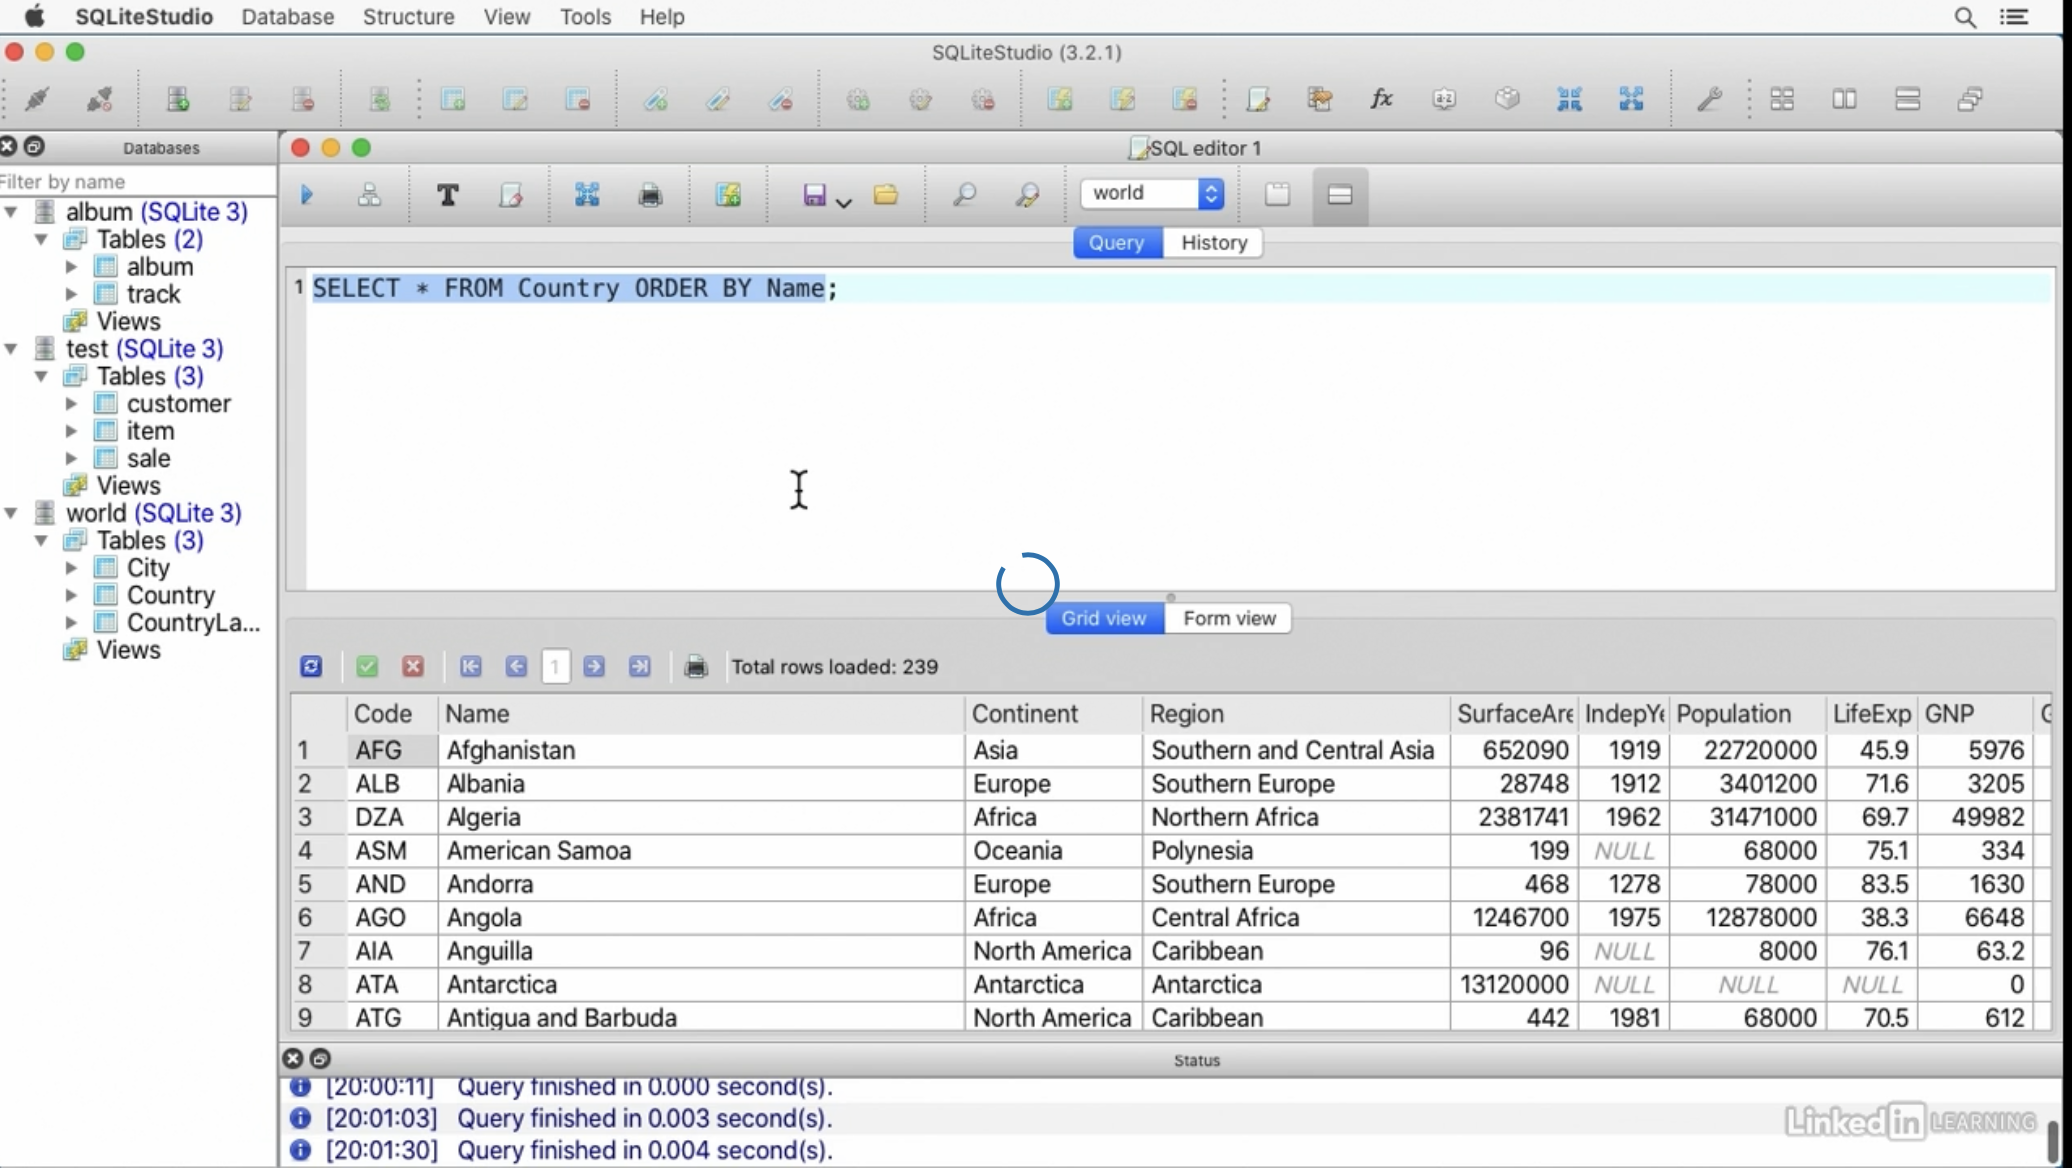
\includegraphics[scale = 0.3]{attachment/chapter_3/Scc043}
	\caption{}
	\label{fig:Scc043}
\end{figure}´

Anstatt * können auch einzelne Spaltennamen adressiert werden.

\begin{lstlisting}[style=SQL]
SELECT		Name, Code
From		Country
Order by	Name;
\end{lstlisting} 
Es wird bei nicht wie bei \gls{g_M} $[...]$ benötigt, um Spalten zu adressieren.

Wie schon erwähnt, soll die Spaltenbezeichnung geändert werden, kann dies für jede einzelne Spalte getan werden.


\begin{lstlisting}[style=SQL]
SELECT		Name AS "Name Neu", Code AS "Country_Code"
From		Country
Order by	Name_Neu;
\end{lstlisting}
In diesem Fall verhält es sich ähnlich wie in \gls{g_M}. Für einen String als Spaltennamen werden Anführungszeichen verwendet.

\begin{lstlisting}[style=SQL]
SELECT		Name AS Name2, Code 
From		Country
Order by	Name2;
\end{lstlisting} 

Mit Hilfe einer Aggregatfunktion können Werte für die gruppierte Spalte ausgegeben werden.

\begin{lstlisting}[style=SQL]
SELECT Count(Quantity), ProductID
FROM OrderDetails
Group by ProductID;
\end{lstlisting}

\begin{figure}[H]
	\centering
	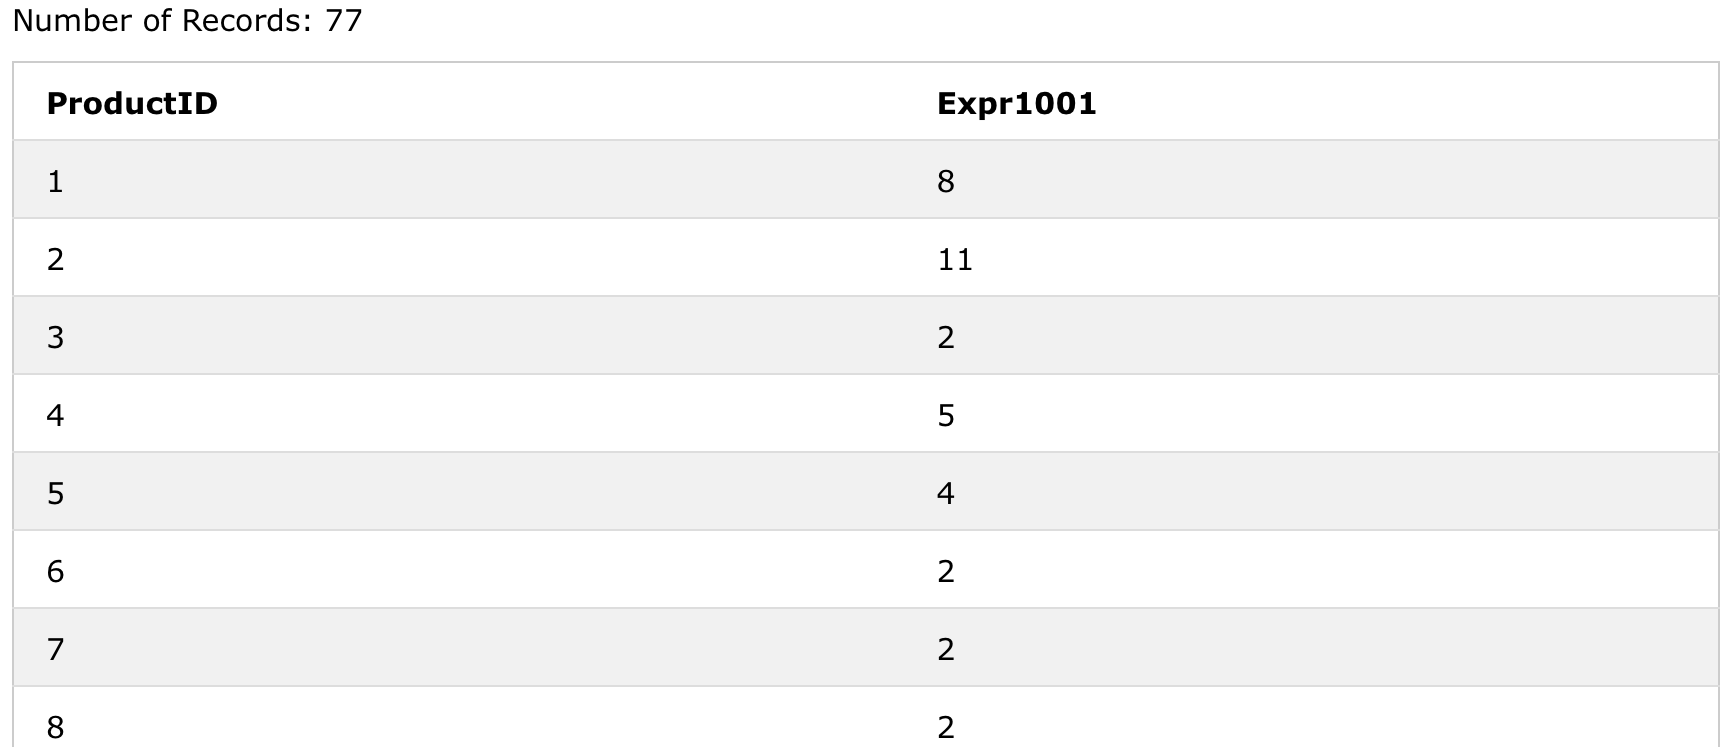
\includegraphics[scale = 0.3]{attachment/chapter_3/Scc051}
	\caption{}
	\label{fig:Scc051}
\end{figure}

Die Anzahl der Aggregationen ist nicht beschränkt.

\begin{lstlisting}[style=SQL]
SELECT SUM(Quantity), Count(ProductID)
FROM OrderDetails
GROUP BY ProductID;
\end{lstlisting}

Zu Vermerken ist, dass nur die Spalten generiert werden, welche auch auch durch \bl{SELECT} ausgewählt werden.

\begin{lstlisting}[style=SQL]
SELECT ProductID, SUM(Quantity) AS SUM_Quantity, Count(ProductID) AS Count_Qunatity
FROM OrderDetails
GROUP BY ProductID;
\end{lstlisting}

\begin{figure}[H]
	\centering
	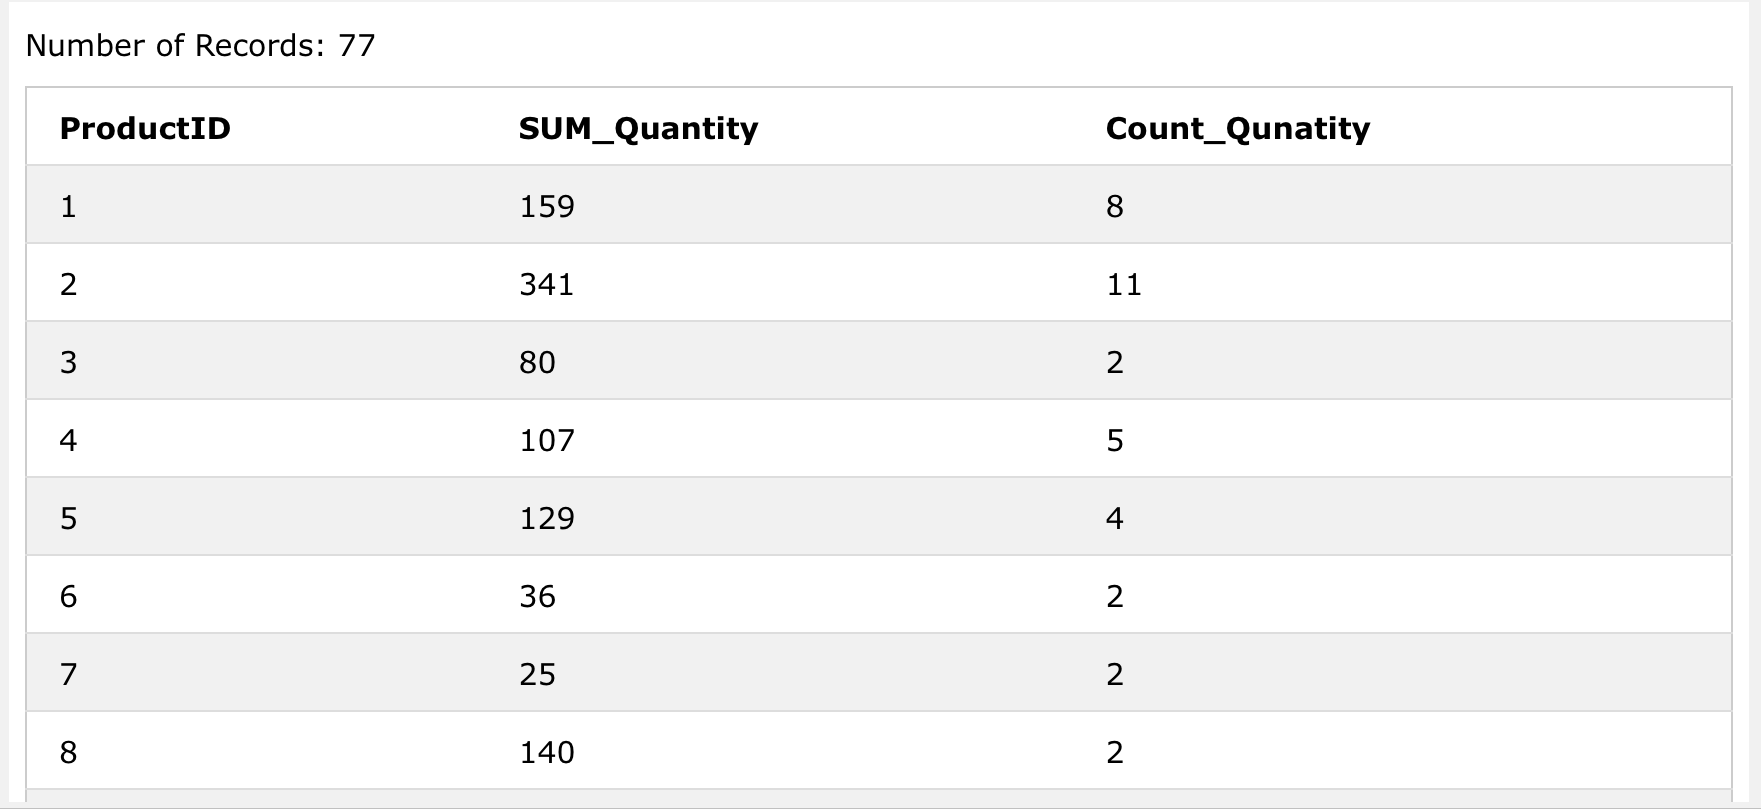
\includegraphics[scale = 0.3]{attachment/chapter_3/Scc053}
	\caption{}
	\label{fig:Scc053}
\end{figure}

\subsubsection{LIMIT - Who many Rows}
Mit dem Ausdruck \bl{Limit} kann die Anzahl der Zeilen reglementiert werden.
Dieser Ausdruck kommt nach \bl{Order BY}.

\begin{lstlisting}[style=SQL]
SELECT 	Name, Contient, Region // column name
From 		County // table name
WHERE		Country = 'Germany'
ORDER BY	Name
LIMIT		5
\end{lstlisting}

\subsubsection{OFFSET - Ausschluss der ersten Zeilen}
Die Auswahl der Zeilen kann auch noch der Indexierung der Tabelle erfolgen.
Mit dem Begriff \bl{OFFSET} wird eine Auswahl der der letzten $m-n$ Zeilen getroffen. Wobei $m$ die Anzahl der gesamten übergeben Tabellenanzahl ist und $n$ der zu reduzierenden Zeilen ist.


\begin{lstlisting}[style=SQL]
SELECT 	Name, Contient, Region // column name
From 		Country // table name
WHERE		Region = 'West'
ORDER BY	Name
OFFSET		5 // Ersten 5 Zeilen werden nicht berücksichtigt.
\end{lstlisting}

\subsection{Concepts}
\subsubsection{Function Types}
Aggregatfunktionen haben die folgende Syntax

\begin{lstlisting}[style=SQL]
SELECT 	Funktiontype(Column) From Table
\end{lstlisting}

\paragraph{Count()}
Die Funktion \bl{Count()} zählt die Zeilen der generierten Tabellen.
Es können dabei zwischen der ganzen Tabelle und einzelnen Spalten unterschieden werden. 
Wählt man einzelnen Spalten aus, werden nicht leere Zeilen gezählt.\\

\bl{Count()} angewandt auf die gesamt Tabelle
\begin{lstlisting}[style=SQL]
SELECT 	Count(*)
From 		Country // table name
\end{lstlisting}

generiert eine Tabelle mit dem Spaltentitel $"$Count(*)$"$, in welcher in der ersten Zeile der gesucht Wert steht.
\begin{figure}[H]
	\centering
	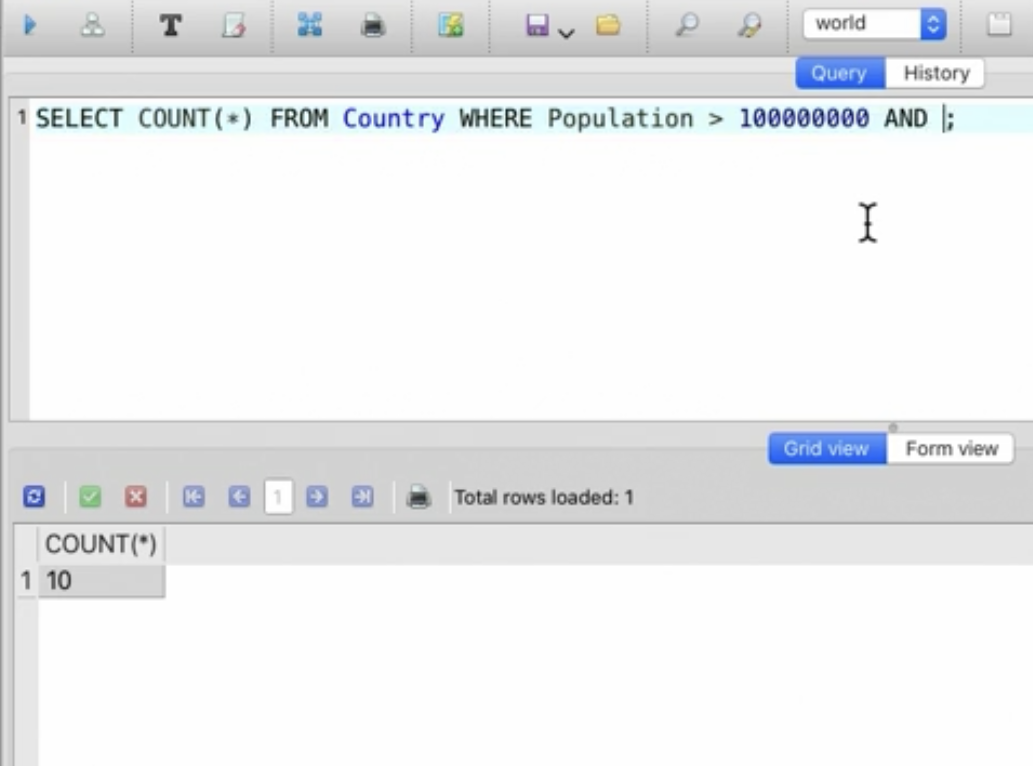
\includegraphics[scale = 0.3]{attachment/chapter_3/Scc046}
	\caption{}
	\label{fig:Scc046}
\end{figure}

Die Einschränkung auf eine gewisse Spalte, gibt die Anzahl der Zeilen, welche nicht null sind, wieder.

\begin{lstlisting}[style=SQL]
SELECT 	Count(Region)
From 		Country 
\end{lstlisting}

Ebenso können weitere Einschränkungen und Überprüfungen an der Tabelle vorgenommen werden.

\begin{lstlisting}[style=SQL]
SELECT 	Count(Region), Contient
From 		Country 
WHERE		Contient = 'Europe'
\end{lstlisting}

Manche Anpassungen haben kein Effekt auf das Ergebnis der Funktion.

\begin{lstlisting}[style=SQL]
SELECT 	Count(*)
From 		Country // table name
ORDER BY	Name
\end{lstlisting}

Sollen unterschiedliche Einträge verglichen werden, wird \bl{DISTINCT} als Zusatz verwendet, siehe \bl{DISTINCT Clause}

\paragraph{Aggregatfunktionen}
Zu den Aggregatfunktion gehört 
\begin{itemize}
\item AVG()
\item MAX(), MIN()
\item SUM(),
\item Count()
\end{itemize}


\subsubsection{DISTINCT Clause}
Innerhalb einer Aggregatfunktion werden werden nur alle ungleichen, nicht leere Zeilen ausgewählt.

In der Funktion \bl{Count()} angewandt, werden nur Zeilen gezählt, welche nicht gleich sind.
\begin{lstlisting}[style=SQL]
SELECT Count(DISTINCT Quantity)
FROM OrderDetails;
\end{lstlisting}

Die Clause kann auch vor einem Spaltennamen in der \bl{SELECT} Clause angewandt werden.

\begin{lstlisting}[style=SQL]
SELECT DISTINCT Quantity
FROM OrderDetails;
\end{lstlisting}

\begin{figure}[H]
	\centering
	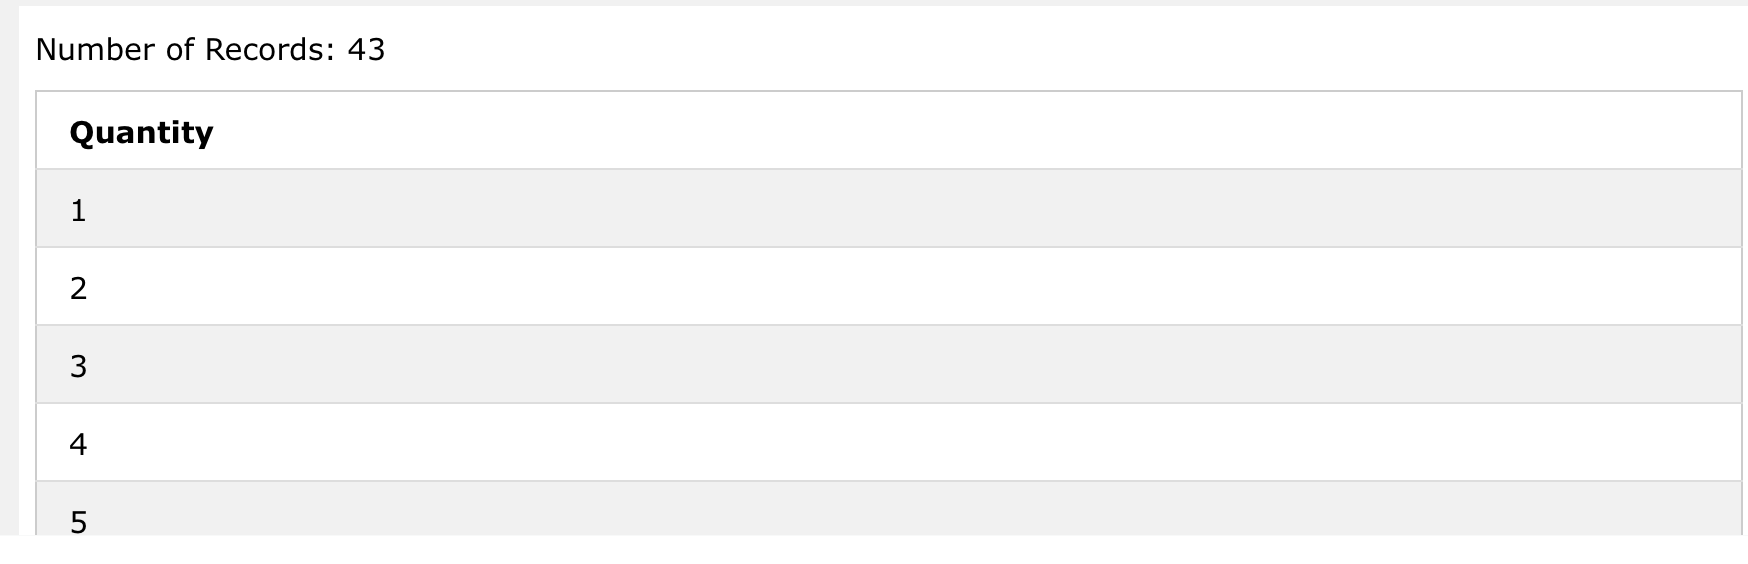
\includegraphics[scale = 0.3]{attachment/chapter_3/Scc054}
	\caption{}
	\label{fig:Scc054}
\end{figure}

Werden weitere Spalten hinzugefügt, bezieht sich die Eindeutigkeit auf die gesamte Zeilenbreite der Tabelle. 

\begin{lstlisting}[style=SQL]
SELECT DISTINCT Quantity, ProductID
FROM OrderDetails;
\end{lstlisting}


\begin{figure}[H]
	\centering
	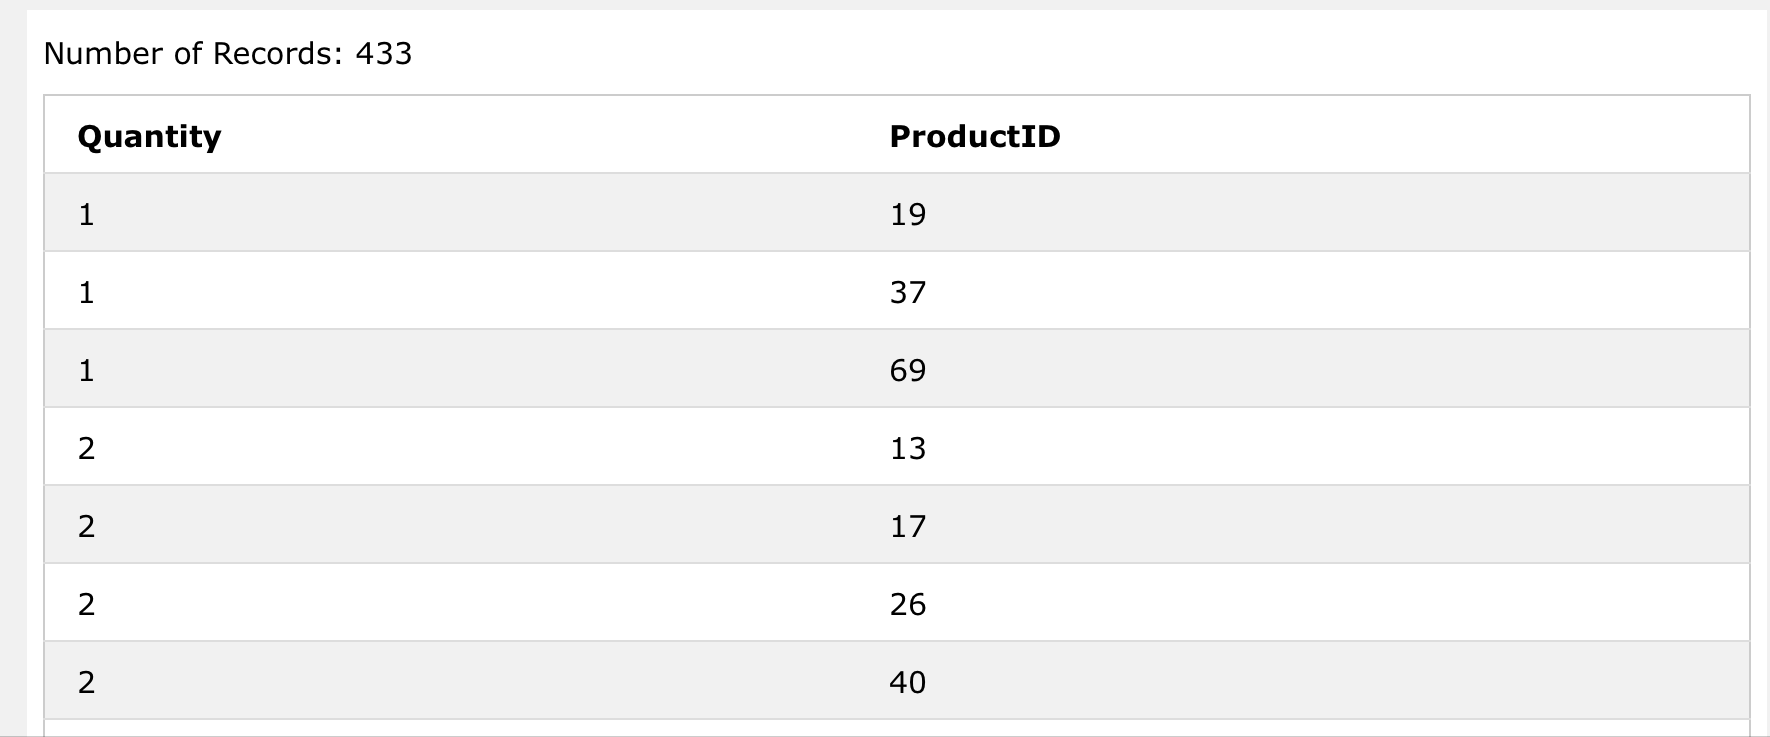
\includegraphics[scale = 0.3]{attachment/chapter_3/Scc055}
	\caption{}
	\label{fig:Scc055}
\end{figure}

Im Vergleich: 
\begin{lstlisting}[style=SQL]
SELECT Quantity, ProductID
FROM OrderDetails
ORDER BY Quantity;
\end{lstlisting}

sind 518 Zeilen geniert worden, hingegen nur 433 unter Berücksichtigung der Eindeutigkeit.
\begin{figure}[H]
	\centering
	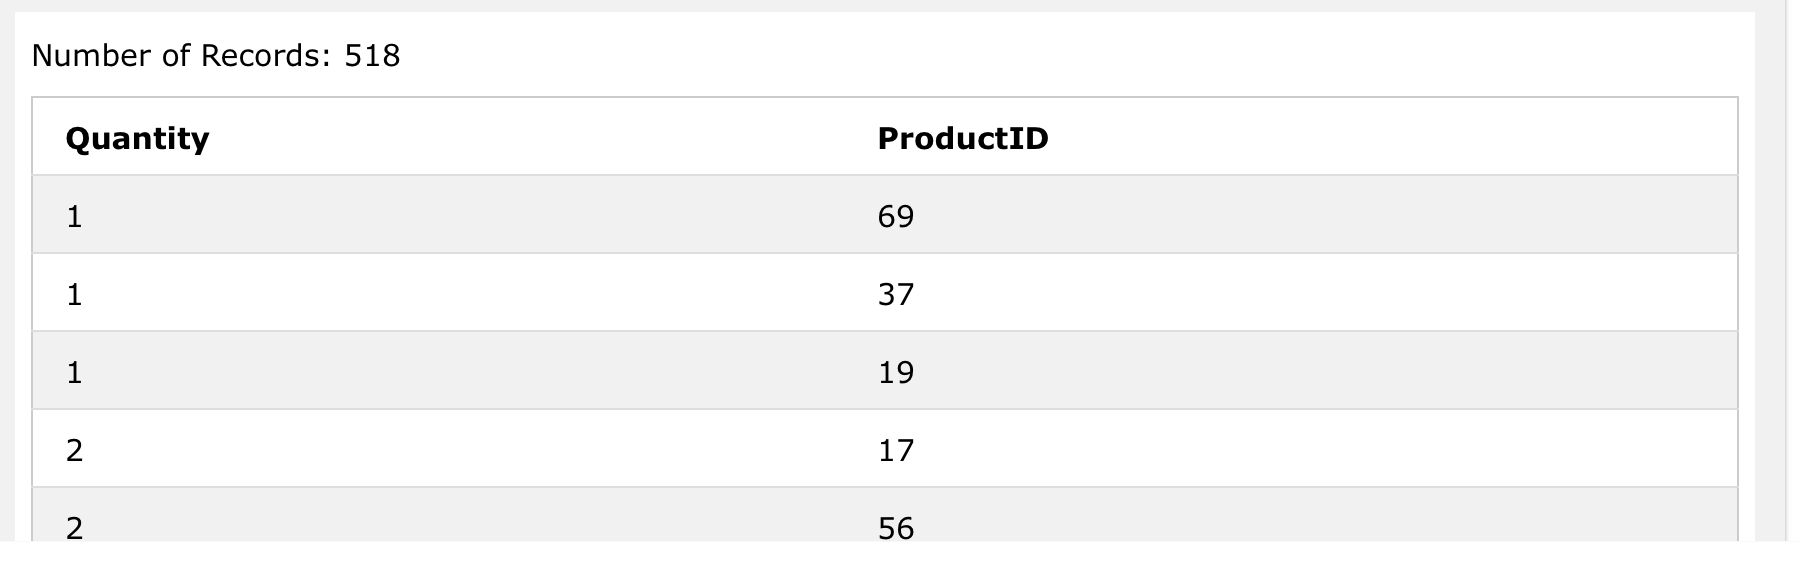
\includegraphics[scale = 0.3]{attachment/chapter_3/Scc056}
	\caption{}
	\label{fig:Scc056}
\end{figure}

\subsubsection{CREATE TABLE ... ()}
Um eine Tabelle zu erstellen, wird \bl{CREATE Table} verwendet.
Die Schema hinter diesem Ausdruck beschreibt die Spaltennamen und Typen.
Dabei wird zu erst der Spaltenname genannt und danach der Typ.


\begin{lstlisting}[style=SQL]
CREATE TABlE Tabellenname (
Spaltenname_1 TEXT,
Spaltenname_2 INTEGER,
Spaltenname_3 BOOLEAN
);
\end{lstlisting}
Neue Werte können über \bl{INSERT INTO} eingepflegt werden.


\begin{lstlisting}[style=SQL]
INSERT INTO Tabellenname
(Spaltenname_1, Spaltenname_2)
Value ('text', 4, True);
\end{lstlisting}

\subsubsection{DROP TABLE ...}
\begin{lstlisting}[style=SQL]
DROP TABLE Test;
\end{lstlisting}

Wenn die Tabelle nicht existiert, kommt es zu einem Fehler. Dieser kann umgangen werden, indem \bl{IF EXISTS} vor dem Tabellennamen geschrieben wird.

\begin{lstlisting}[style=SQL]
DROP TABLE IF EXISTS Test;
\end{lstlisting}

\subsubsection{INSERT INTO ... ()()}
Daten können auch an Tabellen angefügt werden.
Die \bl{INSERT INTO} Clause baut sich in drei Teile auf
\begin{itemize}
\item Tabllenbezug
\item Spaltenbezug
\item Werte
\end{itemize}


\begin{lstlisting}[style=SQL]
INSERT INTO Customers
(Spalten_1, Spalte_2)
VALUE ('Test', 2);
\end{lstlisting}

Wir die Spalte nicht erwähnt, wir der Null-Wert eingesetzt.

\begin{lstlisting}[style=SQL]
INSERT INTO Customers
(Spalte_2)
VALUE (2);
\end{lstlisting}

Werte aus anderen Tabellen können über \bl{SELECT} eingefügt werden.
Anstatt \bl{Value} wird das Select Statement verwendet.

\begin{lstlisting}[style=SQL]
Creat table Test 
(a integer, b text, c text);
INSERT INTO Test
Select ID, Name, Adress From Customer;
Select * From Test;
\end{lstlisting}

\begin{figure}[H]
	\centering
	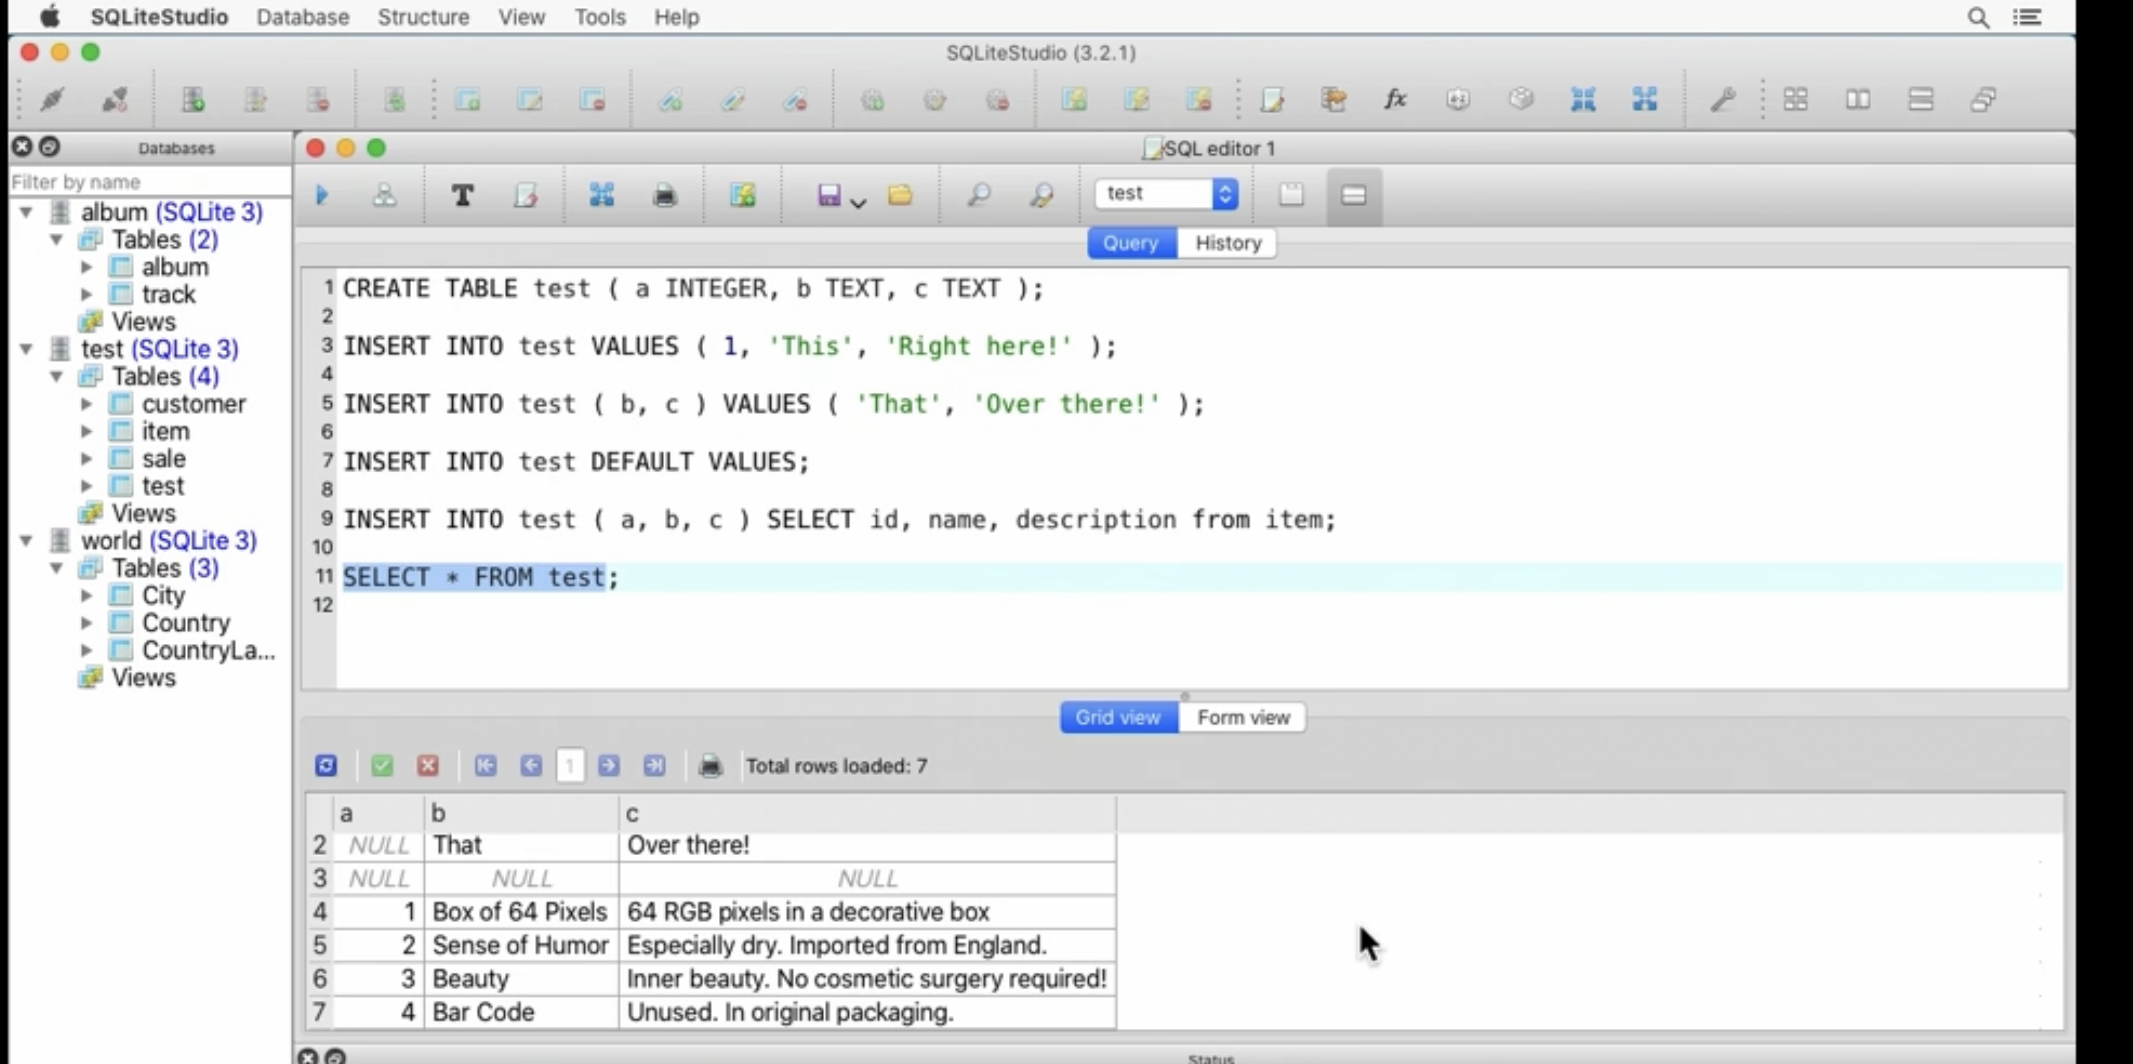
\includegraphics[scale = 0.3]{attachment/chapter_3/Scc057}
	\caption{}
	\label{fig:Scc057}
\end{figure}

\subsubsection{UPDATE ... SET ... WHERE}
Update wirkt auf die gesamte Tabelle. Daher ist es wichtig, die Bedingung oder Bedingungen festzulegen, welche Zeilen direkt angesprochen werden sollen.
Der Aufbaue des Ausdruckes zieht wie folgt aus:
\begin{itemize}
\item Tabllenbezug
\item \bl{SET} Spaltenbezug mit Änderunge
\item \bl{WHERE} Bedingung 
\end{itemize}

\begin{lstlisting}[style=SQL]
UPDATE Customers
SET Spalte_1 = 'Test', Spalte_3 = 'Test'
WHERE Spalte_2 = 'Tesst';
\end{lstlisting}

Wenn keine Bedingung angegeben ist, werden alle Werte in einer spezifischen Spalte geändert.

\begin{lstlisting}[style=SQL]
UPDATE Customers
SET Spalte_1 = 'Test';
\end{lstlisting}

\subsubsection{DELETE FROM ... WHERE}
Unterscheidet sich zu \bl{UPDATE} in der Kategorie, dass ganze Zeilen gelöscht werden, nicht nur einzelne Werte. Dies kann über \bl{UPDATE} erfolgen.

\begin{lstlisting}[style=SQL]
DELETE 
FROM Customers
WHERE id = 5;
\end{lstlisting}

In dem obigen Beispiel wir die Ziele mit Index 5 gelöscht.

\subsubsection{NULL Value} 
Um Zellen auf den Eintrag \bl{null} zu testen, kann in \gls{SQL} nicht nach null gesucht werden. 

\begin{lstlisting}[style=SQL]
WHERE id = null // Gilt nie. Die Tabelle bleibt leer.
\end{lstlisting}

Damit nach \bl{null} Werte gesucht werden kann, muss folgende Überprüfung erfolgen:

\begin{lstlisting}[style=SQL]
WHERE id IS NULL
\end{lstlisting}

Die Negation lautet \bl{IS NOT NULL}.

Diese Beschreibung wird auch verwendet, wenn Datentypen für Spalten festgelegt werden.


\begin{lstlisting}[style=SQL]
CREATE TABLE test (
a Interger NOT NULL,
b Text NOT NULL,
c Text
);

INSERT INTO test Value 
(1, 'abs', 'sde');

INSERT INTO test (b) Values ('asd'); // Ruft einen Fehler hervor, weil a NOT NULL fordert.
\end{lstlisting}

\subsubsection{DEFAULT}
Wie \bl{NOT NULL} kann eine Default Bedingung erstellt werden.
\begin{lstlisting}[style=SQL]
DROP TABlE IF EXIST test;
CREATE TABLE test (
a Interger DEFAULT 0,
b Text NOT NULL,
c Text
);
\end{lstlisting}

\subsubsection{UNIQUE}
Siehe \bl{DEFAULT}

\begin{lstlisting}[style=SQL]
DROP TABlE IF EXIST test;
CREATE TABLE test (
a Interger UNIQUE,
b Text NOT NULL,
c Text
);
\end{lstlisting}

\subsubsection{ALTER TABLE ... ADD}
Um Spalten zu einer Tabelle hinzuzufügen, wird die \bl{ALTER TABLE ... ADD} Funktion verwendet.

\begin{lstlisting}[style=SQL]
CREATE TABLE test (
a Interger UNIQUE,
b Text NOT NULL,
c Text
);

ALTER TABLE test ADD d test;
\end{lstlisting}
Ebenso kann auch hier gleich ein \bl{Default} Wert mit \bl{ADD} d test DEFAULT 'panda' hinterlegt werden.

\subsubsection{CASE - Conditional Expression}
Um einen Werte in einer Spalte zu überprüfen, kann \bl{CASE} verwendet werden.
Im einfachen Fall wird eine Überprüfung der Werte einer Spalte durchgeführt. Mit \bl{CASE} können mehrer Abfragen gestellt werden. Das Resultat kann in die gleiche Spalte oder eine andere geschrieben werden.

Die Werte, die gespeichert werden sollen, werden unter \bl{End} abgespeichert.
Der Aufbau der Funktion ist.

\begin{lstlisting}[style=SQL]
CASE (Spalte) WHEN (Bewertung) THEN (...)
ELSE (...)
END (Speicherort)
\end{lstlisting}

\begin{lstlisting}[style=SQL]
SELECT department, salary, name
CASE department WHEN 50 THEN 1,5*salary
WHEN 60 THEN 2,0*salary
END 'Finaly_Salary' 
From Employee;
\end{lstlisting}

\begin{figure}[H]
	\centering
	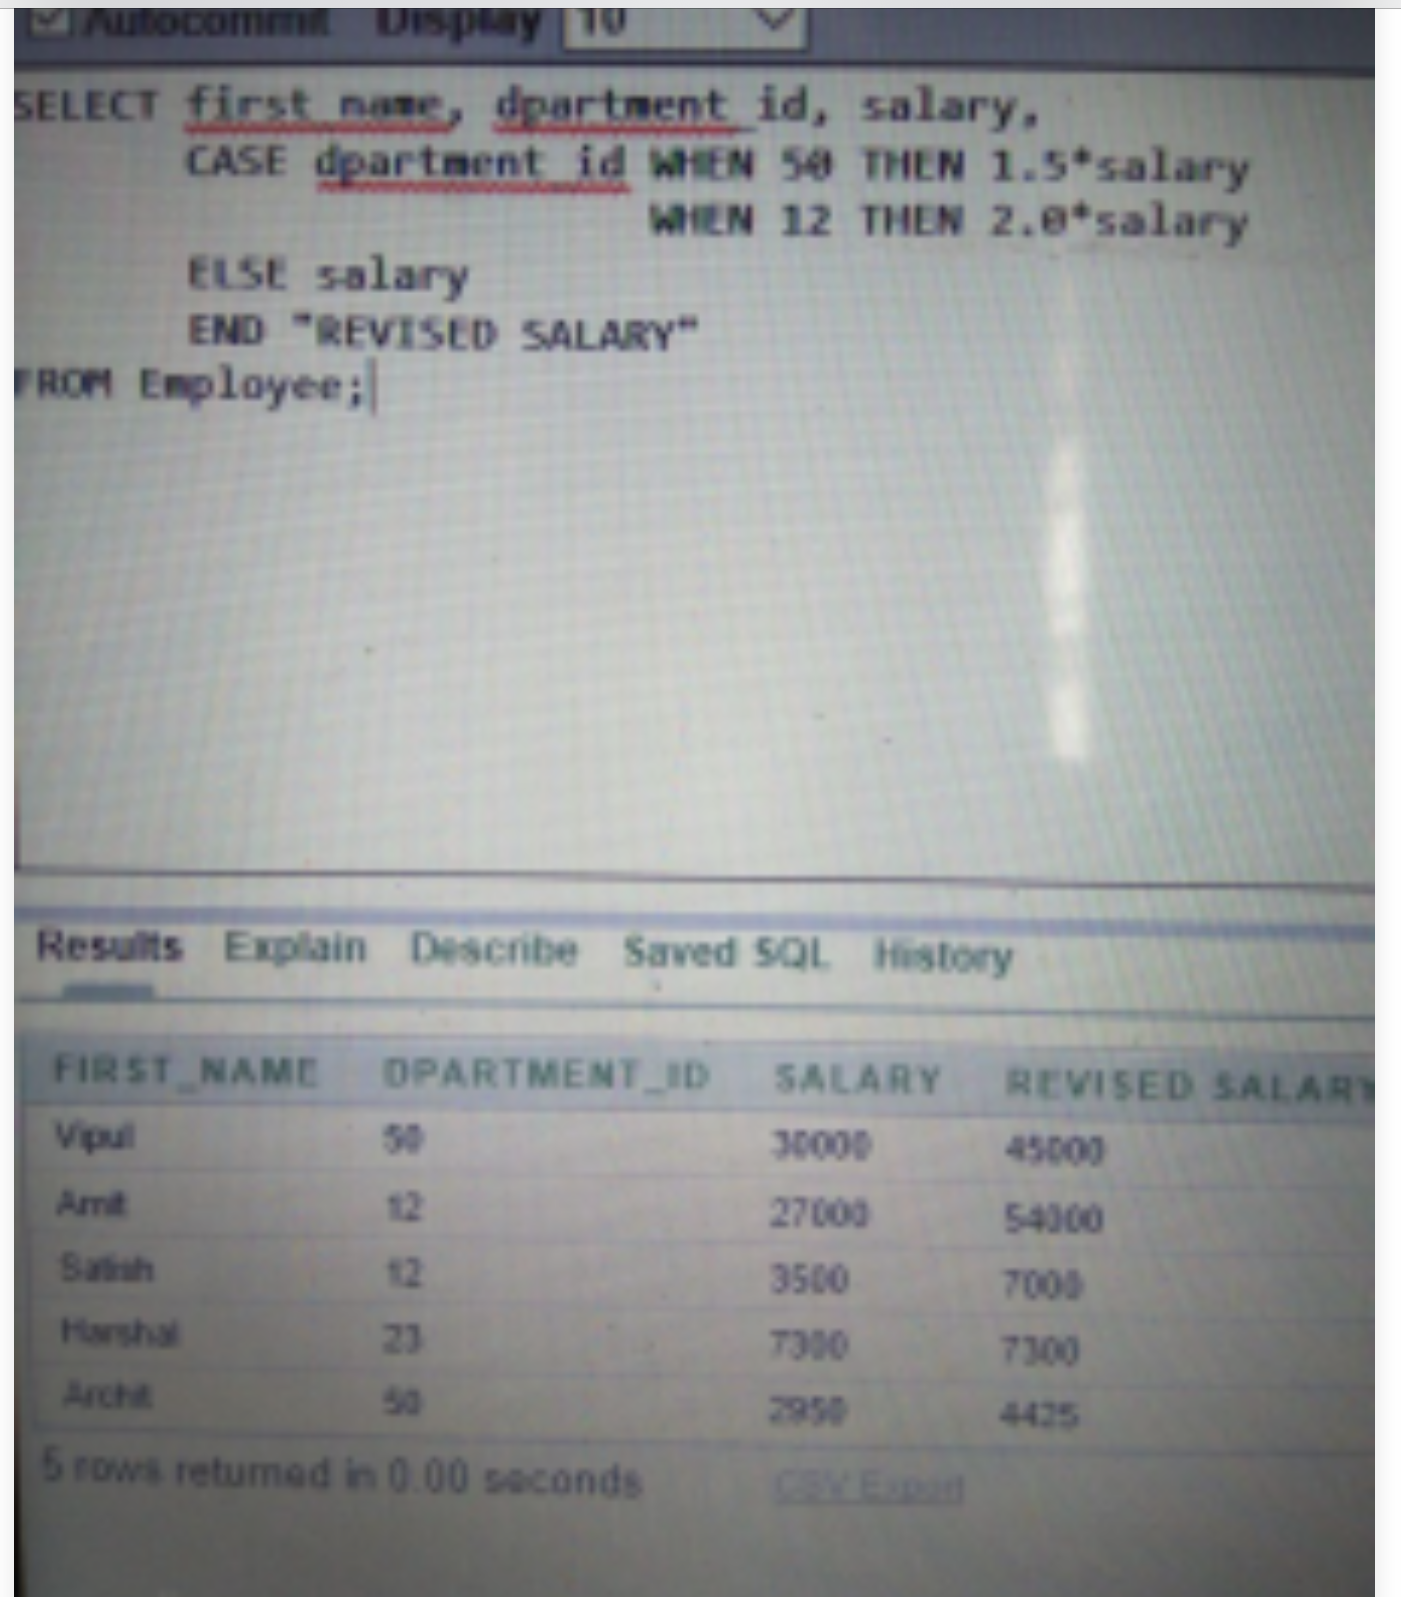
\includegraphics[scale = 0.3]{attachment/chapter_3/Scc059}
	\caption{}
	\label{fig:Scc059}
\end{figure}

Die Funktion lässt zwei Möglichkeiten zu:
\begin{itemize}
	\item \begin{lstlisting}[style=SQL]
	CASE (Spalte) WHEN (Bewertung) THEN (...)
	ELSE (...)
	END AS (Neuer Speicherort)
	\end{lstlisting}
	\item \begin{lstlisting}[style=SQL]
	CASE WHEN (Spalten bezogene Bewertung) THEN (...)
	ELSE (...)
	END AS (Neuer Spaltenname)
	\end{lstlisting}
\end{itemize}
\subsubsection{Ansteuern von Spalten}
In \gls{g_SQLite} wird die Syntax $[]$ für Spalten verwandt. Dabei können Spaltennamen auch ohne Eckige Klammern geschrieben werden, wenn der Tabellennamen angegeben wird.
 
 \begin{lstlisting}[style=SQL]
	SELECT Substr([a],1,2)
	From t;
	-- oder
	SELECT Substr(a,1,2)
	From t;
 \end{lstlisting}

\subsection{Joints}
Die Relationsfunktion fußen auf den bestehenden Relation der Mengenlehre.\\

\subsubsection{Join on or more tables}
Die Joins sind wie folgt aufgebaut:
\begin{itemize}
	\item Select aller Spalten die angezeigt werden sollen. Dabei können die Spalten aus den verbundenen Tabellen angesteuert werden. Ebenso können auch die Spalten der zugrundeliegenden Tabelle angezeigt werden. 
	\begin{itemize}
		\item Jede Tabelle kann einzeln eingesteuert werden $Tabellenname$. Die Auswahl der Spalten erfolgt über den Operator $.$. 
		\item Die Möglichkeit alle Spalten anzusprechen erfolgt ebenso den bekannten Operator $*$. 
		\begin{lstlisting}[style=SQL]
			Select customer.name AS "Customer-Name", item.name AS "Item-Name", sale.*
		\end{lstlisting}
	\end{itemize}
	\item Mit \bl{From} wird die zugrundeliegende Tabelle angesteuert.
	\item Es können jetzt mehrere \bl{Joins} angefügt werden. Der Aufbau eines \bl{Joins} ist, dass an Ersterstelle die Angefügt Tabelle steht. Danach wir festgelegt, über welchen Schnittpunkt die Tabellen verbunden werden.
	\begin{lstlisting}[style=SQL]
	Join customer ON sale.customer_id = customer.id
	Join item ON sale.item_id = item.id;
	\end{lstlisting}
	\item Weiter Funktionalitäten können angefügt werden
		\begin{lstlisting}[style=SQL]
	WHERE sale.id = 2;
	\end{lstlisting}
\end{itemize}
Mit Joinsfunktion erlaubt so, dass verschiedene Datensätze verbunden werden.
	\begin{lstlisting}[style=SQL]
	--Ziel ist es die Namen aus der customer Tabelle zu laden.
	Select customer.name AS "Customer-Name", item.name AS "Item-Name", sale.*
	From sale
	Join customer ON sale.customer_id = customer.id
	Join item ON sale.item_id = item.id
	;
	\end{lstlisting}
\begin{figure}[H]
	\centering
	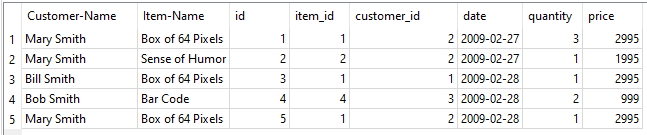
\includegraphics[scale = 0.6]{attachment/chapter_3/Scc060}
	\caption{}
	\label{fig:Scc060}
\end{figure}

\subsubsection{Kinds of Joins}
\begin{figure}[H]
	\centering
	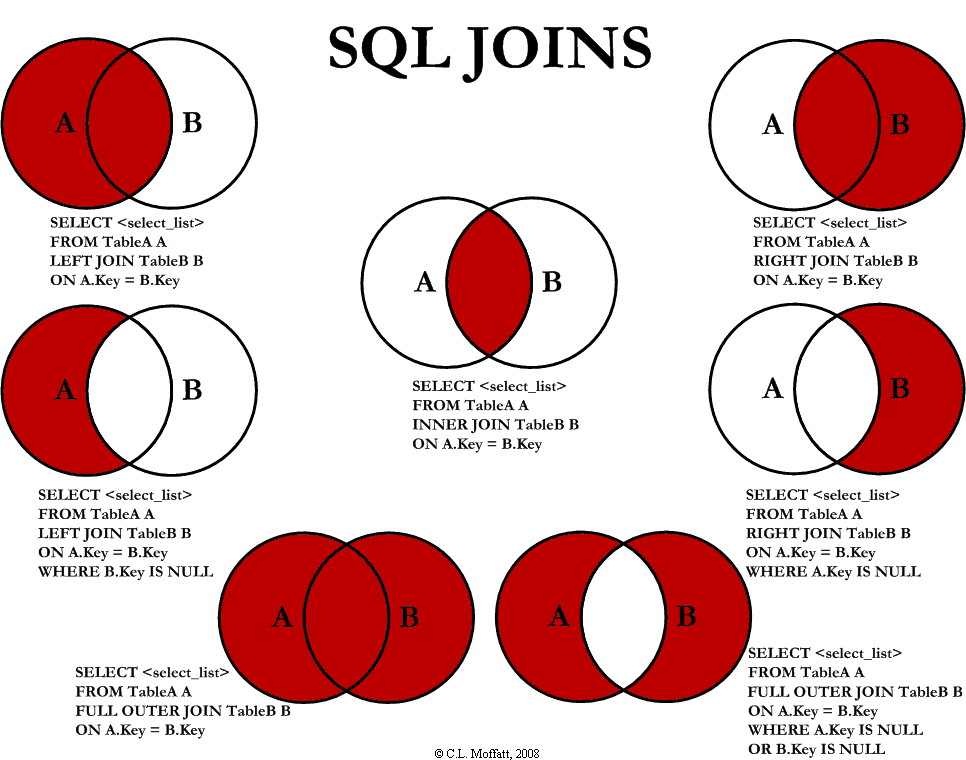
\includegraphics[scale = 0.3]{attachment/chapter_3/Scc061}
	\caption{}
	\label{fig:Scc061}
\end{figure}

\subsection{Selection of Function}
\subsubsection{Find the lenght of a string}
Die Funktion \bl{LENGTH()} gibt die Länge eines String-Values wieder.
\begin{lstlisting}[style=SQL]
-- Bestimmen der Länge einer Spalte: Leerzeichen werden auch mitgezählt.
Select id, name, Length(name) AS 'Länge der Spalte Name'
From customer
; 
\end{lstlisting}

\begin{figure}[H]
	\centering
	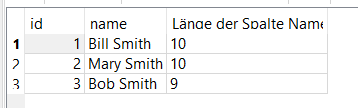
\includegraphics[scale = 0.6]{attachment/chapter_3/Scc062}
	\caption{}
	\label{fig:Scc062}
\end{figure}

\subsubsection{Substring of Field of Date}
Datumseinträge können in Teil Einträge zerlegt werden.
\begin{lstlisting}[style=SQL]
Select date, 
	Substr(date,1,4) AS Year,
	Substr(date,6,2) AS Month,
	Substr(date,9,2) AS Day
From sale
;
\end{lstlisting}
\begin{figure}[H]
	\centering
	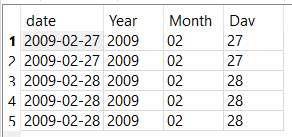
\includegraphics[scale = 0.6]{attachment/chapter_3/Scc063}
	\caption{}
	\label{fig:Scc063}
\end{figure}



\subsubsection{Count()- Group by (aggregate function)}
Die \bl{Count()} Funktion auf eine Spalte oder eine Tabelle zählt die nicht leeren Einträge. Angewandt auf eine Tabelle, wir die Anzahl der Zeilen dargestellt. Erst mit der \textbf{Kombination} \bl{Group by} wirkt die Funktion wie ein Funktion, welche ein Parameter übergeben bekommen wird. \\

\paragraph{Count(), Group by - same coloum}
Für jeden aggregierte Eintrag (grouped), wir die Anzahl ermittelt. Ohne dies zählt die \bl{Count()} Funktion nur die Zeilen einer Tabelle.
	\begin{lstlisting}[style=SQL]
	Select state, Count(state)
	From customer
	Group by state
	;
\end{lstlisting}

\paragraph{Count(), Group by - different coloum}
Die \bl{Count()} Funktion funktioniert, nicht anders, wenn sie auf eine spezifische Spalte angewandt wird. Die Funktion zählt nur die aggegierten Zeilen, für jede Tabelle.
	\begin{lstlisting}[style=SQL]
	Select state, Count(address) -- Wie viel unterschiedliche Adress gibt es in jedem Staat.
	From customer
	Group by state
	;
\end{lstlisting}

\subsubsection{Mix}
\begin{description}
	\item[Trim] Die Trim-Funktionen werden weiter unterteilt. Der Kern ist, dass entweder Leerzeichen oder andere Zeichen aus dem Textfeld eintfernt werden. Dabei unterscheidet \bl{Trim()} in linksseitige \bl{LTrim} und rechtseitige \bl{RTrim} Funktionen.
	\item[Case Function] Strings können in groß oder klein Darstellung der ASCI-Zeichen umgewandet werden. 
	\item Typeof() gibt den Typ des Eintrages wieder.
	\item[Datetime] Die \bl{Datetime()} Funktion nimmt als Input Variablen \textit{Strings}. Das aktuelle Datum wir mit $'now'$ beschrieben.
	\begin{lstlisting}[style=SQL]
		Select Datetime('now','+1 day'),
	\end{lstlisting}
\end{description}

\subsection{Transaction}
Zugriffe auf die Datenbank können in Packete geschnürt werden. Diese Transaktionen Starten und Enden mit einem Befehl. Dieser kann sich von SQL Datenbanksystem zu Datenbanksystem anders sein. 
Transaktionspackete sichern
\begin{itemize}
	\item Daten Integrität
	\item Performance
\end{itemize}

In SQLite gilt
\begin{lstlisting}[style=SQL]
	Begin Transaction;
	...
	End Transaction;
\end{lstlisting}

Geht etwas schiff, oder werden bestimmt Kriterien nicht erfüllt, so kann mit \bl{Rollback} die bisherige Transaktion rückgängig gemacht werden. 
\begin{lstlisting}[style=SQL]
	Begin Transaction;
	...
	Rollback;
	...
	End Transaction;
\end{lstlisting}

Als Beispiel dient die folgende Übung:
\begin{lstlisting}[style=SQL]
-- 02 transactions
-- test.db

CREATE TABLE widgetInventory (
id INTEGER PRIMARY KEY,
description TEXT,
onhand INTEGER NOT NULL
);

CREATE TABLE widgetSales (
id INTEGER PRIMARY KEY,
inv_id INTEGER,
quan INTEGER,
price INTEGER
);

INSERT INTO widgetInventory ( description, onhand ) VALUES ( 'rock', 25 );
INSERT INTO widgetInventory ( description, onhand ) VALUES ( 'paper', 25 );
INSERT INTO widgetInventory ( description, onhand ) VALUES ( 'scissors', 25 );

SELECT * FROM widgetInventory;
SELECT * FROM widgetSales;

BEGIN TRANSACTION;
INSERT INTO widgetSales ( inv_id, quan, price ) VALUES ( 1, 5, 500 );
UPDATE widgetInventory SET onhand = ( onhand - 5 ) WHERE id = 1;
END TRANSACTION;

BEGIN TRANSACTION;
INSERT INTO widgetInventory ( description, onhand ) VALUES ( 'toy', 25 );
ROLLBACK;
SELECT * FROM widgetInventory;
\end{lstlisting}

\subsection{Triggers}
Triggers erlauben bestimmt Aktionen durchzuführen, wenn ein Ereignis an einer Tabelle durchgeführt wird. Die verschiedenen Trigger werden in SQLite an die Tabelle angefügt.
\begin{figure}[H]
	\centering
	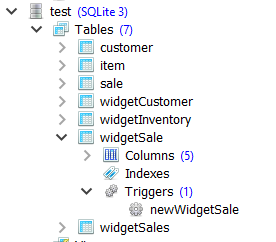
\includegraphics[scale = 0.6]{attachment/chapter_3/Scc064}
	\caption{}
	\label{fig:Scc064}
\end{figure}

Ein Trigger wird mit dem Namen, den Auslöser und den Bezug initialisiert.
\begin{lstlisting}[style=SQL]
	Create TRIGGER [name] [Event] ON [Tabelle]
		Begin
		...
		End
	;
\end{lstlisting}

Im gewählten Beispiel ist der Auslöser das Einfügen einer neuen Zeile.
\begin{lstlisting}[style=SQL]
	Create TRIGGER NewCustomerID After INSERT ON widgetSales
		Begin
			UPDATE widgetCustomer -- Die zu modifizierte Tabelle
			SET last_order_id = NEW.id -- New. Ist das Objekt, welche generiert wird, wenn eine neue Zeile in widgetSales eingelegt wird.
			WHERE widgetCustomer.id = NEW.customer_id --
			;
		End
	;
\end{lstlisting}

Die Trigger Funktion kann verwendet werden, für das Ergänzen von Daten. Diese können Beispielsweise nach dem Einfügen einer Zeile ausgelöst werden.

\begin{lstlisting}[style=SQL]
-- 01 update triggers
-- test.db
Drop Table if exists widgetSale;
Drop Table if exists widgetCustomer;

CREATE TABLE widgetCustomer ( id INTEGER PRIMARY KEY, name TEXT, last_order_id INT, stamp TEXT);
CREATE TABLE widgetSale ( id INTEGER PRIMARY KEY, item_id INT, customer_id INT, quan INT, price INT, stamp TEXT);

INSERT INTO widgetCustomer (name) VALUES ('Bob');
INSERT INTO widgetCustomer (name) VALUES ('Sally');
INSERT INTO widgetCustomer (name) VALUES ('Fred');

SELECT * FROM widgetCustomer;
Select * From widgetSale;

CREATE TRIGGER stampSale After Insert ON widgetSale
BEGIN
UPDATE widgetSale SET stamp = Datetime('now') WHERE id = NEW.id;
UPDATE widgetCustomer Set last_order_id = New.id, stamp = DateTime('now')
Where widgetCustomer.id = New.customer_id;
END
;

INSERT INTO widgetSale (item_id, customer_id, quan, price) VALUES (1, 3, 5, 1995);
INSERT INTO widgetSale (item_id, customer_id, quan, price) VALUES (2, 2, 3, 1495);
INSERT INTO widgetSale (item_id, customer_id, quan, price) VALUES (3, 1, 1, 2995);
SELECT * FROM widgetSale;
SELECT * FROM widgetCustomer;
\end{lstlisting}
Was zu beachten ist, dass der \textbf{Trigger} selbst ausgeführt werden muss. Dabei wird dieser in unter 
\begin{figure}[H]
	\centering
	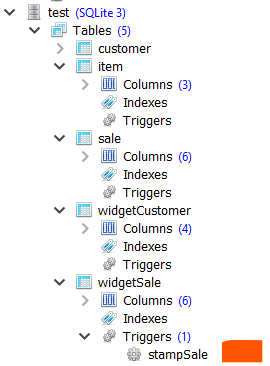
\includegraphics[scale = 0.6]{attachment/chapter_3/Scc065}
	\caption{}
	\label{fig:Scc065}
\end{figure}
abgespeichert.
Das Objekt \textbf{NEW} steuert den Record der letzten Zeile der vorgegebenen Tabelle, in dem Fall \textit{widgetSale}.
Die Spalten werden dann als Attribute des Objektes \textbf{New} gesehen.

\subsection{Subselects}
Abfragen können ebenfalls als temporäre Tabelle betrachtet werden.
\begin{lstlisting}[style=SQL]
	CREATE TABLE t ( a TEXT, b TEXT );
	INSERT INTO t VALUES ( 'NY0123', 'US4567' );
	INSERT INTO t VALUES ( 'AZ9437', 'GB1234' );
	INSERT INTO t VALUES ( 'CA1279', 'FR5678' );
	SELECT * FROM t;
	
	-- Trennen der Strings
	SELECT SUBSTR([a],1,2) AS State, 
	SUBSTR([b],1,2) AS Country,
	SUBSTR([a],3) As State_Code,
	SUBSTR([b],3) AS Country_Code
	From t;
	
	Select * From Country;
	
	--  Suche Country-Name mit SELECT als Tabelle
	SELECT Country.Name, st.Country_Code
	From (SELECT SUBSTR([a],1,2) AS State, 
	SUBSTR([b],1,2) AS Country,
	SUBSTR([a], 3) As State_Code,
	SUBSTR([a], 3) AS Country_Code
	From t) AS st
	Join Country
	On Country.Code2 = st.Country;
	
	DROP TABLE t;
\end{lstlisting}

\subsubsection{IN Operator}
Mit dem In-Operator können mehrere Bedingungen geprüft werden. Das bedeutet
\begin{lstlisting}[style=SQL]
	SELECT *
	From Country
	WHERE Name IN(Deutschland, Japan, Frankreich); -- Die Syntax ist nicht = In(...)
\end{lstlisting} 

In der Spalte [Name] wird nach den Werten \textit{Deutschland, Japan} oder \textit{Frankreich} gesucht. Das gleiche Ergebnis ist auch erreicht, wenn zwei \textbf{OR} Operatoren verwendet werden würden.
Mit Subselect kann eine Liste als Speicherort für multiple Bedingungen verwendet werden.

\begin{lstlisting}[style=SQL]
	SELECT *
	From Country
	WHERE Code2 IN((SELECT SUBSTR([b],1,2) AS Country_Code, SUBSTR([b],1,1))
	From t))
	;
\end{lstlisting}
Die Bezugstabelle muss als Liste vorliegen. Das bedeutet, eine Tabelle kann nicht vom IN() Operator verwendet werden.

\subsubsection{View - temporay table}
Subselect können in View gespeichert werden. Diese befinden sich als Unterpunkt unter \textbf{Tabellen}. 

	\begin{figure}[H]
	\centering
	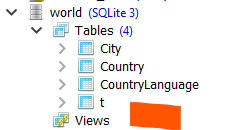
\includegraphics[scale = 0.3]{attachment/chapter_3/Scc066}
	\caption{}
	\label{fig:Scc066}
\end{figure}
Über \textit{Drop View Beispielname} werden diese entfernt. Der Befehl zur Generierung sieht wie folgt aus: 
\begin{lstlisting}[style=SQL]
	CREATE VIEW view_name AS
	SELECT column1, column2, ...
	FROM table_name
	WHERE condition;
\end{lstlisting}

Beispiel \textit{track}:
\begin{figure}[H]
	\centering
	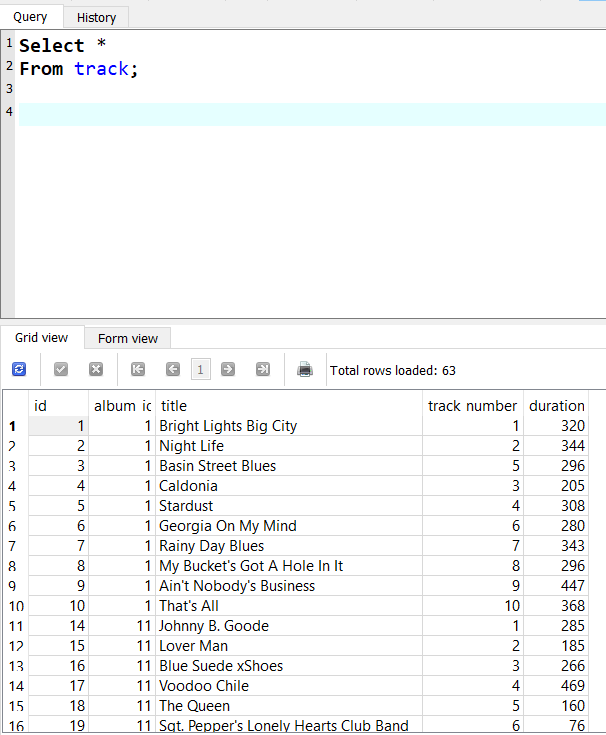
\includegraphics[scale = 0.3]{attachment/chapter_3/Scc067}
	\caption{}
	\label{fig:Scc067}
\end{figure}

Die Bewertung der Dauer wird in der View Tabelle \textit{DurationView} gespeichert.
